\begin{refsection} 
 
\chapter{Density Functional Theory} \label{chapter:dft}
 
\setlength{\epigraphwidth}{4in} 
\epigraph{\textit{``The underlying physical laws necessary for the 
mathematical theory of a large part of physics and the whole of chemistry are 
thus completely known, and the difficulty is only that the exact application 
of these laws leads to equations much too complicated to be soluble. It 
therefore becomes desirable that approximate practical methods of applying 
quantum mechanics should be developed, which can lead to an explanation of the 
main features of complex atomic systems without too much computation.''}}{Paul 
Dirac} 
\vspace{2em} 
 
\setlength{\epigraphwidth}{4in} 
\epigraph{\textit{``When teaching chemistry students, I explain that \gls{DFT} is 
some algorithm meaning unreliable, while ab initio is Latin for too 
expensive."}}{Kieron Burke} 
\vspace{3em} 
 
Density functional theory (\gls{DFT}) is a popular quantum mechanical 
method for calculating the electronic structure of a system, based on the idea 
that all of the relevant information on the electrons is stored in the 
electron density function. Within this theory, the properties of the system 
are defined as functionals, i.e. ``a function of a function", of the electron 
density. It is one of the most widely used \textit{ab initio} methods 
available, mainly because of its wide range of possible applications as well 
as its relative computational simplicity.  
 
In this chapter, I discuss the theoretical underpinnings of \gls{DFT}. 
Section~\ref{dft:sec-theory} describes the many-body problem and explains the 
theoretical framework that allows us to tackle electronic structure 
calculations using \gls{DFT}. Section~\ref{dft:sec-computational} continues by 
explaining the important concepts of practical computations, such as the basis
set for the expansion of the one-electron orbitals and the pseudopotential method. 
Section~\ref{dft:sec-linear} discusses 
linear response theory and the calculation of the dielectric tensor. Finally, 
the chapter finishes with a brief summary of transition state theory in 
Section~\ref{dft:sec-transition}, as well as the nudged elastic band method, 
which is a valuable technique for determining the kinetic barrier of 
transitions.  
 
\newpage 
 
\section{Theoretical Background} \label{dft:sec-theory} 
 
We start our discussion by considering the quantum many-body problem. A 
crystal can be described by the wave function of the interacting particles, 
consisting of M nuclei and N electrons~\cite{Springborg2017}: 
\begin{equation} 
 \Psi (\mathbf{r}_1, \sigma_1, \hdots,\mathbf{r}_N, \sigma_N, \mathbf{R}_1, 
\Sigma_1, \hdots, \mathbf{R}_M, \Sigma_M), 
\end{equation} 
where the many-body wave function $\Psi$ depends on the position and spin 
coordinates of the electrons ($\mathbf{r}_i,\sigma_i$) with mass $m_e$ and the 
nuclei ($\mathbf{R}_k,\Sigma_k$) with mass $M_k$. In the interest of making 
the equations manageable, it is conventional to write the coordinates as: 
\begin{eqnarray*} 
&(\mathbf{r}_1, \sigma_1, \hdots,\mathbf{r}_N, \sigma_N) = 
(\mathbf{x}_1,\hdots , \mathbf{x}_N) = \mathbf{x} 
\\&(\mathbf{R}_1, \Sigma_1, \hdots, \mathbf{R}_M, \Sigma_M) = 
(\mathbf{X}_1,\hdots , \mathbf{X}_M) = \mathbf{X}. 
\end{eqnarray*} 
Using this notation, the time-independent Schr\"odinger equation becomes 
\begin{equation} 
\hat{H} \Psi (\mathbf{X}, \mathbf{x}) = E \Psi (\mathbf{X}, \mathbf{x}). 
\end{equation} 
In the non-relativistic case, the 
Hamiltonian of the many-body problem is given by 
\begin{equation} 
\begin{gathered} 
\hat{H}=-\sum_{k=1}^M \frac{\hbar^2}{2M_k}\Delta_{\mathbf{R}_k}-\sum_{j=1}^N 
\frac{\hbar^2}{2m_e} \Delta_{\mathbf{r}_j} + \frac{1}{2} \sum_{k_1 \neq k_2 = 
1}^M \frac{1}{4 \pi \varepsilon_0} \frac{Z_{k_1} Z_{k_2} e^2 
}{|\mathbf{R}_{k_1}-\mathbf{R}_{k_2}|} \\ + \frac{1}{2} \sum_{j_1 \neq j_2 = 
1}^N \frac{1}{4 \pi \varepsilon_0} \frac{e^2 
}{|\mathbf{r}_{j_1}-\mathbf{r}_{j_2}|} - \sum_{k=1}^M \sum_{j=1}^N  \frac{1}{4 
\pi \varepsilon_0} \frac{Z_k e^2 }{|\mathbf{R}_{k}-\mathbf{r}_{j}|}, 
\end{gathered} 
\end{equation} 
where $Z_k$ is the number of protons in the nuclei, $\varepsilon_0$ is the 
vacuum permittivity and $\hbar$ is the reduced Planck constant. The first two 
terms correspond to the kinetic energy of the nuclei and the electrons. The 
other three terms describe the potential energy for the nucleus-nucleus, 
electron-electron and the nucleus-electron interaction. In order to further 
shorten future notation, we write the Hamiltonian terms as 
\begin{equation} 
\hat{H} = \hat{H}_{k,n} + \hat{H}_{k,e} + \hat{H}_{p,n-n} + \hat{H}_{p,e-e} + 
\hat{H}_{p,n-e}, 
\end{equation} 
where $\hat{H}_{k,n}$, $\hat{H}_{k,e}$ are the kinetic energy terms and 
$\hat{H}_{p,n-n}$, $\hat{H}_{p,e-e}$, $\hat{H}_{p,n-e}$ are the potential 
energy terms for the corresponding interactions. 
 
\subsection{The Born-Oppenheimer Approximation} 
 
Our first step in tackling the many-body problem is the Born-Oppenheimer 
approximation~\cite{Born1927}. Since the mass of a nucleus is much larger than 
that of an electron, it is reasonable to assume that the nuclei move much more 
slowly than the electrons. As such, we can consider their position to be 
fixed, with the electrons reacting instantly to any change in the nuclear 
positions. Applying these assumptions leads to the following approximate 
expression for the wave function: 
\begin{equation} 
\Psi (\mathbf{X}, \mathbf{x}) = \Psi_n (\mathbf{X}) \Psi_e (\mathbf{X}, 
\mathbf{x}). 
\end{equation} 
The nuclear wave function $ \Psi_n (\mathbf{X})$ depends solely on the nuclear 
coordinates, whereas the electronic wave function $\Psi_e 
(\mathbf{X},\mathbf{x})$ depends directly on the electronic coordinates and 
considers the nuclear coordinates as parameters. If we substitute this product 
of wave functions into the Schr\"odinger equation and divide by the total wave 
function, we find 
\begin{equation} 
\frac{(\hat{H}_{k,e} + \hat{H}_{p,e-e} + \hat{H}_{p,n-e})\Psi_e(\mathbf{X}, 
\mathbf{x})}{\Psi_e(\mathbf{X}, \mathbf{x})} = E - \frac{(\hat{H}_{k,n} + 
\hat{H}_{p,n-n})\Psi_n (\mathbf{X})}{\Psi_n (\mathbf{X}) }. 
\end{equation} 
 
The right hand side of this equation is a function that only depends on the 
nuclear coordinates $\mathbf{X}$. If we write this function as 
$E_e(\mathbf{X})$ and multiply both sides with the electronic wave function, 
we find the Schr\"odinger equation for the electrons: 
\begin{equation} 
(\hat{H}_{k,e} + \hat{H}_{p,e-e} + \hat{H}_{p,n-e})\Psi_e(\mathbf{X}, 
\mathbf{x}) = E_e(\mathbf{X}) \Psi_e(\mathbf{X}, \mathbf{x}). 
\end{equation} 
We can see that the electronic wave function only depends parametrically on 
the nuclei coordinates, through the electrostatic interaction in 
$\hat{H}_{p,n-e}$. Changing to atomic units 
\begin{equation}\label{dft:eq-atomic} 
\hbar = 1 \hspace{0.3in} m_e = 1\hspace{0.3in} e  = 1 \hspace{0.3in} 4 \pi 
\varepsilon_0 = 1, 
\end{equation}  
we finally obtain the electronic Schr\"odinger equation: 
\begin{equation}\label{dft:eq-elecSch} 
\begin{gathered} 
\left[ -\frac{1}{2}\sum_{i=1}^N \Delta_{\mathbf{r}_i} + \frac{1}{2} \sum_{i_1 
\neq i_2 = 1}^N \frac{1}{|\mathbf{r}_{i_1}-\mathbf{r}_{i_2}|} - \sum_{k=1}^M 
\sum_{i=1}^N \frac{Z_k}{|\mathbf{R}_{k}-\mathbf{r}_{i}|} \right] 
\Psi_e(\mathbf{X}, \mathbf{x}) = E_e(\mathbf{X}) \Psi_e(\mathbf{X}, 
\mathbf{x}). 
\end{gathered} 
\end{equation} 
 
The Born-Oppenheimer approximation significantly reduces the complexity of the 
many-body problem. Every set of fixed nuclei coordinates defines an external 
potential, for which we can solve the Schr\"odinger equation to obtain the 
electronic wave function. However, since the nuclei coordinates are considered 
to be fixed parameters, solving Eq.~(\ref{dft:eq-elecSch}) does not provide any 
information on the lattice constants or atomic positions. We return to this 
issue in Section.~\ref{dft:sec-hellmann}.
 
\subsection{Hohenberg-Kohn Theorems}\label{dft:sec-HKtheorems} 
 
Although the idea of using the electron density as the main variable when 
solving the many-body problem dates from the 1920's, it was not properly 
formalized until 1964. This is when Hohenberg and Kohn introduced two theorems 
that formulate density functional theory as an exact theory of many-body 
systems~\cite{Hohenberg1964}. We begin our discussion of these theorems by 
defining the electron density function as 
\begin{equation} 
\rho(\mathbf{r}) = \bra{\Psi_e} \hat{\rho} (\mathbf{r}) \ket{\Psi_e}, 
\end{equation} 
where $\hat{\rho} (\mathbf{r})$ is the electron density operator: 
\begin{equation} 
\hat{\rho} (\mathbf{r}) = \sum_{i=1}^{N} \delta (\mathbf{r}_i - \mathbf{r}). 
\end{equation}
and the electron density is normalized to the number of electrons:
\begin{equation}
\int \rho (\mathbf{r}) d\mathbf{r} = N
\end{equation}
 
The first of the Hohenberg-Kohn theorems states that there is a one to one 
correspondence between the ground state density and the external potential of 
our system. When solving the electronic Schr\"odinger equation for a certain 
external potential, we find the unique ground state wave function, which can 
in turn be used to calculate the ground state density. Because of the first 
Hohenberg-Kohn theorem, we know that the reverse is possible as well. In other 
words, we cannot have two different external potentials for a given electron 
density $\rho(\mathbf{r})$. This means that the electron density contains all 
the relevant information of the system. As a result, we can write any 
observable as a unique functional of the electron 
density~\cite{Cottenier2013}: 
\begin{equation} 
O[\rho] = \bra{\Psi} \hat{O} \ket{\Psi}. 
\end{equation} 
 
The second Hohenberg-Kohn theorem concerns the functional of the electronic 
energy $E_e[\rho]$. It states that the form of this functional is given by 
\begin{equation}\label{dft:eq-elenergy} 
E_e[\rho] = F_{HK}[\rho] + \int \rho(\mathbf{r}) V_{ext}(\mathbf{r}) 
d\mathbf{r}, 
\end{equation} 
where $F_{HK}[\rho]$ is called the Hohenberg-Kohn energy functional and 
$V_{ext}(\mathbf{r})$ is the external potential generated by the nuclei: 
\begin{equation} 
V_{ext}(\mathbf{r}) =  - \sum_{k=1}^M 
\frac{Z_k}{\left|\mathbf{R}_{k}-\mathbf{r}\right|}. 
\end{equation} 
Furthermore, once we know the functional of the electronic energy, we can 
approximate the ground state energy by using a variational principle: 
\begin{equation} 
E_0 = E_e[\rho_0] \leq E_e[\rho], 
\end{equation} 
with $\rho_0$ the ground state density of the electrons. Hence, if we know the 
functional $F_{HK}[\rho]$, we can provide an upper bound\footnote{Since we use 
a variational principle, the electron energy found by minimization is in 
principle an upper bound for the ground state electron energy. However, when 
approximations are used for the functional $F_{HK}[\rho]$, the minimized 
electron energy can no longer be considered an upper bound. This means that it 
is possible that \gls{DFT} calculations produce a ground state energy below $E_0$.} 
for the ground state energy by inserting different functions for 
$\rho(\mathbf{r})$ and looking for the minimal value of Eq. 
(\ref{dft:eq-elenergy}). 
 
An important concept in this discussion is the \textit{universality} of the functional 
$F_{HK}[\rho]$. The second Hohenberg-Kohn theorem does not simply propose the 
existence of an energy functional $F_{HK}[\rho]$ for each external potential 
$V_{ext}(\mathbf{r})$, it declares that there is one such functional which is 
the same for every system. Unfortunately, we do not know the exact form of 
this functional, which means that we have to look for approximations. We know 
that $F_{HK}[\rho]$ consists of the kinetic and the interaction energy of the 
electrons: 
\begin{equation}\label{dft:eq-HKfunctional} 
F_{HK}[\rho] = T[\rho] + \frac{1}{2} \iint 
\frac{\rho(\mathbf{r})\rho(\mathbf{r'})}{\left| \mathbf{r} - 
\mathbf{r'}\right|} d\mathbf{r} d\mathbf{r'} + E_{xc}'[\rho],  
\end{equation} 
where the first term denotes the kinetic energy, the second term is due to the 
Coulomb interaction, and all other interaction energy is combined in the 
\textit{exchange-correlation} energy $E_{xc}'[\rho]$. Finding a good 
expression for $E_{xc}'[\rho]$ is of great importance for \gls{DFT} calculations, 
and is discussed in more detail in Section~\ref{dft:sec-functionals}. 
 
The Hohenberg-Kohn theorems, as presented in this section, apply to the ground 
state of a system of spin-unpolarised electrons subjected to an external 
potential. However, they can be extended to include the presence of several 
types of particles. In order to study a spin-polarised system, we separate the 
electron density in a component for the spin-up orbitals and the spin-down 
orbitals~\cite{Martin2004}: 
\begin{equation} 
\rho(\mathbf{r}) = \rho(\mathbf{r},\sigma = \hspace{0.05in}\uparrow) + 
\rho(\mathbf{r}, \sigma = \hspace{0.05in}\downarrow). 
\end{equation} 
This results in a new functional for the electron energy, which now also 
depends on the spin density $s(\mathbf{r}) = \rho(\mathbf{r},\sigma = 
\hspace{0.05in}\uparrow) - \rho(\mathbf{r}, \sigma = 
\hspace{0.05in}\downarrow)$: 
\begin{equation} 
E_e = E_e[\rho(\mathbf{r}),s(\mathbf{r})] = E_e^s[\rho^s(\mathbf{x})], 
\end{equation} 
where in the final expression $\rho^s(\mathbf{x})$ is a function that depends 
on both the electrons' position and spin coordinates.  
 
\subsection{Kohn-Sham Equations} \label{dft:sec-kohn_sham} 
 
The Hohenberg-Kohn theorems turn the electron density into the fundamental 
variable of the system. The first Hohenberg-Kohn theorem guarantees that no 
information is lost when we consider the electron density as the main variable 
instead of the wave function. The second Hohenberg-Kohn theorem allows us to 
use a variational principle to find the ground state electron density.  
 
The next step in solving the many-body problem using \gls{DFT} was introduced by 
Kohn and Sham in 1965~\cite{Kohn1965}. They considered a system of 
non-interacting electrons that has exactly the same energy and electron 
density as the original problem. This fictitious system is subject to a 
different external potential\footnote{Note that for spin-polarised systems, 
the effective potential can also depend on the spin coordinates.} 
$V_{eff}(\mathbf{r})$, but has a much simpler expression for the electron 
energy functional: 
\begin{equation}\label{dft:eq-nonE} 
E_{e}'[\rho] = T_0[\rho] + \int V_{eff}(\mathbf{r}) \rho(\mathbf{r}) 
d\mathbf{r}, 
\end{equation} 
where $T_0[\rho]$ is the kinetic energy of the new system, which differs from 
$T[\rho]$. Since the particles are now non-interacting, the Hamiltonian has 
the form 
\begin{equation} 
\hat{H}_{KS} = \sum_{i=1}^{N} \left[ - \frac{1}{2} \Delta_{\mathbf{r_i}} + 
V_{eff}(\mathbf{r}) \right]. 
\end{equation} 
For this Hamiltonian, the solution of the Schr\"odinger equation can be 
written as a Slater determinant: $\Psi_e'(\mathbf{r})~=~\left| 
\phi_1(\mathbf{r}),\phi_2(\mathbf{r}), \hdots , \phi_N (\mathbf{r})\right|$, 
where the single-particle orbitals $\phi_i(\mathbf{r})$ are solutions of the 
single-particle Schr\"odinger equations: 
\begin{equation}\label{dft:eq-KS} 
\left[- \frac{1}{2} \Delta_{\mathbf{r}_i} + V_{eff}(\mathbf{r}) \right] \phi_i 
(\mathbf{r}) = \epsilon_i\phi_i (\mathbf{r}). 
\end{equation} 
The electron density is now given by~\cite{Argaman2002} 
\begin{equation}\label{dft:eq-density} 
\rho(\mathbf{r}) = \sum_{i=1}^N \left|\phi_i(\mathbf{r})\right|^2.
\end{equation} 
 
This non-interacting system is easier to solve, but we do not know 
$V_{eff}(\mathbf{r})$. However, we do know that by definition both systems 
have the same energy and electron density, which can be used to find an 
expression for $V_{eff}(\mathbf{r})$. Writing down the original many-body 
electron energy functional using Eq.~(\ref{dft:eq-HKfunctional}): 
\begin{eqnarray*} 
E_e[\rho] &=& F_{HK}[\rho] + \int \rho(\mathbf{r}) V_{ext}(\mathbf{r}) 
d\mathbf{r} 
\\ &= &T[\rho] + \frac{1}{2} \iint 
\frac{\rho(\mathbf{r})\rho(\mathbf{r'})}{\left| \mathbf{r} - 
\mathbf{r'}\right|} d\mathbf{r} d\mathbf{r'} + \int \rho(\mathbf{r}) 
V_{ext}(\mathbf{r}) d\mathbf{r} + E_{xc}'[\rho], 
\end{eqnarray*} 
we can equate it to the non-interacting total energy from Eq. (\ref{dft:eq-nonE}) 
and rewrite it to find 
\begin{equation}\label{dft:eq-Veff1} 
\int \rho(\mathbf{r}) V_{eff}(\mathbf{r}) d\mathbf{r} = \int \rho(\mathbf{r}) 
V_{ext}(\mathbf{r}) d\mathbf{r} + \frac{1}{2} \iint 
\frac{\rho(\mathbf{r})\rho(\mathbf{r'})}{\left| \mathbf{r} - 
\mathbf{r'}\right|}d\mathbf{r}d\mathbf{r'} + E_{xc}[\rho], 
\end{equation} 
where we have redefined the exchange correlation energy by including the 
difference between the kinetic energy of the original and non-interacting 
system: 
\begin{equation} 
E_{xc}[\rho] = (T[\rho] - T_0[\rho]) + E_{xc}'[\rho]. 
\end{equation} 
Finally, if we take the functional derivative of Eq. (\ref{dft:eq-Veff1}), we get 
an expression for the effective potential: 
\begin{eqnarray} 
V_{eff}(\mathbf{r}) &=& V_{ext}(\mathbf{r}) + \int \frac{\rho 
(\mathbf{r})}{\left| \mathbf{r} - \mathbf{r'} \right|} d\mathbf{r'} + 
\frac{\delta E_{xc}}{\delta \rho} 
\\ \label{dft:eq-Veff}&=& V_{ext}(\mathbf{r}) + V_{H}(\mathbf{r}) + 
V_{xc}(\mathbf{r}), 
\end{eqnarray} 
where $V_H(\mathbf{r})$ is the Hartree or Coulomb potential and 
$V_{xc}(\mathbf{r})$ is the exchange-correlation potential. 
 
We call Eqs. (\ref{dft:eq-KS}), in combination with the expression for 
$V_{eff}(\mathbf{r})$ from Eq. (\ref{dft:eq-Veff}), the \textit{Kohn-Sham} (\gls{KS}) 
equations. At first glance, we seem to be faced with a problem: In order to 
calculate the ground state electron density $\rho(\mathbf{r})$, we need to 
solve the \gls{KS} equations to find the one electron wave functions 
$\phi_i(\mathbf{r})$. However, these equations require the knowledge of the 
effective potential $V_{eff}(\mathbf{r})$, whose calculation in turn requires 
the ground state density $\rho(\mathbf{r})$. To solve this issue, we perform 
what is called a self-consistent field (\gls{SCF}) procedure. Starting from 
an initial guess for the electron density, we calculate the effective 
potential. Once we have the effective potential, we insert it into the 
Kohn-Sham equations to calculate the one electron wave functions. We then use 
these wave functions to calculate the new ground state density, from which we 
can once again derive a new effective potential. This provides us with an 
algorithm which converges to the ground state density after a sufficient 
amount of iterations. This algorithm is shown schematically in Figure 
\ref{dft:fig-scf_cycle}.  

\begin{figure}[ht]  
\centering 
\begin{tikzpicture}[node distance=2em] 
 
    % Nodes 
    \node (1) [box] {Start with trial electron density \\ 
$\rho_0(\mathbf{r})$}; 
    \node (2) [box, below=of 1] {Calculate effective potential \\[4pt] 
                                 $V_{eff}(\mathbf{r}) = V_{ext}(\mathbf{r}) + 
V_{H}(\mathbf{r}) + V_{xc}(\mathbf{r})$}; 
    \node (3) [box, below=of 2] {Solve Kohn-Sham equations \\ 
                                 $\left[- \frac{1}{2} \Delta_{\mathbf{r}_i} + 
V_{eff}(\mathbf{r}) \right] \phi_i (\mathbf{r}) = \epsilon_i\phi_i 
(\mathbf{r}).$}; 
    \node (4) [box, below=of 3] {Calculate new electron density \\ 
                                 $\rho_n(\mathbf{r}) = \sum_{i=1}^N \left| 
\phi_i (\mathbf{r}) \right|^2$}; 
    \node (5) [box, right=of 4] {Solution is converged?}; 
    \node (6) [box, below=3 em of 5] {SCF solution is found \\ 
                                 $\rho(\mathbf{r}) = \rho_n(\mathbf{r})$}; 
 
    % Arrows 
    \draw [->, arrow] (1.south) -- (2.north); 
    \draw [->, arrow] (2.south) -- (3.north); 
    \draw [->, arrow] (3.south) -- (4.north); 
    \draw [->, arrow] (4.east) -- (5.west); 
    \draw [->, arrow] (5.south) -- node [fill=white] {Yes} (6.north); 
    \coordinate (no) at ($(5.north) - (3em, 0)$); 
    \draw [->, arrow] (no) -- node [fill=white] {No} (2 -| no) -- (2.east); 
     
    % Help Boxes 
    \node (help1)[helpbox, above right=-3em and 3 em of 1] {The trial electron 
density is usually constructed from a superposition of the atomic electron 
densities.}; 
    \draw [helpline] (1.east |- help1.west) -- (help1.west); 
    \node (help2)[helpbox, above right=3em and -5em of 5] {A natural choice 
for the convergence condition is the self-consistency of the electron density. 
However, several codes use the difference in energy between SCF steps.}; 
    \coordinate (h2_anchor) at ($(5.north) + (3em, 0)$); 
    \draw [helpline] (h2_anchor) -- (h2_anchor |- help2.south); 
 
\end{tikzpicture} 

\caption{\label{dft:fig-scf_cycle} Flowchart representing the self consistent field 
calculation used to find the ground state density in \gls{DFT} calculations.} 
\end{figure} 
 
The \gls{SCF} procedure is converged when the electron density is 
\textit{self-consistent}, i.e. solving the Kohn Sham equations using the 
effective potential for the converged electron density results in the same 
density. However, several implementations of the \gls{DFT} formalism consider the 
difference between the total electronic energy of two \gls{SCF} iteration steps for 
the convergence criterion. 
 
\subsection{Exchange Correlation Functional} \label{dft:sec-functionals} 
 
The Kohn-Sham method is in principle exact, up to a certain precision 
determined by a parameter in the convergence procedure. However, we are still 
faced with one of the fundamental challenges of \gls{DFT}: the expression of the 
exchange-correlation functional $E_{xc}[\rho]$ is unknown. Since the calculation of the effective potential for each iteration step requires this functional, we 
are forced to make use of approximations. One popular way of classifying the 
various approximations for the exchange-correlation energy is as rungs on 
Jacob's ladder for \gls{DFT}~\cite{Perdew2001}, ultimately leading to chemical 
accuracy heaven (Fig.~\ref{dft:fig-jacob}). These rungs are also often referred to 
as the \textit{level} of the theory. 
 
\begin{figure}[ht]
\centering 
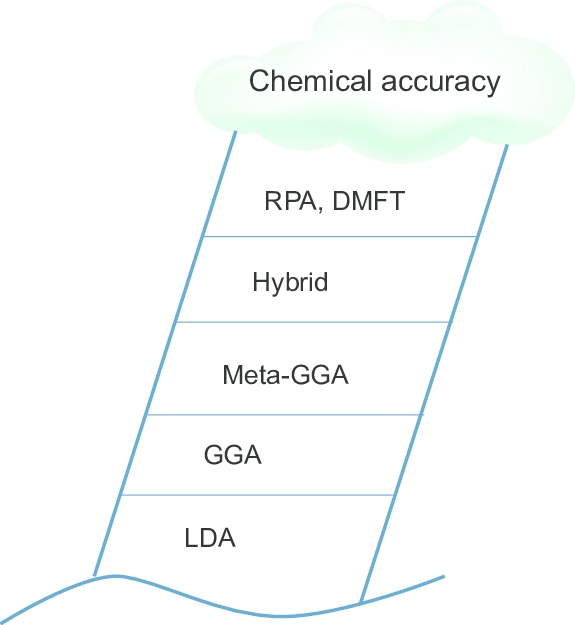
\includegraphics[width=0.5\textwidth]{\figurepath/dft/jacob.png} 
\caption{Jacob's ladder of density functional approximations for the 
exchange-correlation energy. Taken from~\cite{Wang2014}.} 
\label{dft:fig-jacob} 
\end{figure} 
 
The first rung on Jacob's ladder is the local density approximation 
(\gls{LDA}), introduced in the original paper of Kohn and Sham~\cite{Kohn1965}: 
\begin{equation} 
E_{xc}^{LDA}[\rho] = \int \rho(\mathbf{r}) 
\epsilon_{xc}(\rho(\mathbf{r}))d\mathbf{r}, 
\end{equation} 
where $\epsilon_{xc}(\rho(\mathbf{r}))$ is the exchange-correlation energy 
function, which in the \gls{LDA} is assumed to depend only on the electron density 
$\rho(\mathbf{r})$. Most successful variants of the \gls{LDA} calculate the 
exchange-correlation for the homogeneous electron gas, based on an exact 
expression for the exchange part and quantum Monte Carlo simulations for the 
correlation part. 
 
\phantomsection \label{dft:sec-GGA}
In the next level of theory, some non-locality is introduced through the 
gradient of the electron density. In this way, we obtain the 
generalised gradient approximation (\gls{GGA})~\cite{Perdew1992}: 
\begin{equation} 
E_{xc}^{GGA}[\rho] = \int \rho(\mathbf{r}) f(\rho(\mathbf{r}),\left| \nabla 
\rho\right|)d\mathbf{r}, 
\end{equation} 
where $f(\rho(\mathbf{r}),\left| \nabla \rho\right|)$ is a function of the 
electron density $\rho(\mathbf{r})$ and its gradient $\left| \nabla 
\rho\right|$. \gls{GGA}'s generally produce better results than the \gls{LDA}, but 
there is some freedom in determining how exactly the gradient is included in 
the approximation through the definition of $f(\rho(\mathbf{r}),\left| \nabla 
\rho\right|)$. Some variants of the \gls{GGA} use empirical data to fit the 
functional parameters to a wide range of experimental results~\cite{Becke1988, Keal2004}. Alternatively, the functional form and parameters can be constructed based on theoretical constraints. An example of such a 
non-empirical \gls{GGA} functional that is very popular in solid state physics is the 
\textit{Perdew-Burke-Ernzerhof} (\gls{PBE})~\cite{Perdew1996} functional: 
\begin{equation} 
E_{xc}^{PBE}[\rho] = \int \rho(\mathbf{r}) \left[ 
\epsilon_{xc}(\rho(\mathbf{r})) + H[\rho,t] \right] d\mathbf{r}, 
\end{equation} 
with 
\begin{equation} 
H[\rho,t] = \left( \frac{e^2}{a_0} \right) \gamma \phi^3 \text{ln} \left\{ 1 + 
\frac{\beta}{\gamma} t^2 \left[ \frac{1 + A t^2}{1 + A t^2 + A^2 t^4} \right] 
\right\}, 
\end{equation} 
where $t = \left| \nabla \rho \right|/(2 k_s\rho)$ is a dimensionless density 
gradient, with $k_s$ the Thomas-Fermi screening wave number, $a_0$ the Bohr 
radius and $\beta$, $\gamma$ constants\footnote{$\beta = 0.066725$ and $\gamma 
= 0.031091$~\cite{Kohanoff2006}.}. The function A has the following form: 
\begin{equation} 
A = \frac{\beta}{\gamma} \left[ e^{-\epsilon_{xc}(\rho(\mathbf{r}))/(\gamma 
e^2 /a_0)} - 1 \right]^{-1}. 
\end{equation} 

\phantomsection \label{dft:sec-metaGGA}
The next natural extension of the theory includes a dependency on $\nabla^2 
\rho(\mathbf{r})$, which leads to the third rung on Jacob's ladder: 
meta-GGA's. However, this term is also commonly used for functionals that 
include a dependence on the local kinetic energy density: 
\begin{equation} 
\tau (\mathbf{r}) = \sum_{i=1}^N \frac{1}{2} \left| \nabla \phi_i (\mathbf{r}) 
\right|^2 
\end{equation} 
A recent meta-GGA functional based on the local kinetic energy density that 
has been shown to perform well with regard to the cohesive energies and 
lattice parameters of solids is the strongly constrained and appropriately 
normed (\gls{SCAN})~\cite{Sun2015} functional. 
 
\phantomsection \label{dft:sec-hybrid} 
Although many \gls{LDA}, \gls{GGA} and meta-GGA functionals are quite effective at 
calculating the lattice parameters, atomic positions and binding energies, a 
common problem when using these functionals is that they tend to significantly 
underestimate the band gap of semiconductor materials~\cite{Tran2007}. 
Moreover, as they are often based on the homogeneous electron gas, they 
provide a poor description of the electronic structure of \textit{d} and 
\textit{f} valence orbitals, which are usually more localized~\cite{Bengone2000}. 
In order to improve the value of the band gap and localization of 
electrons, it is possible to mix the \gls{DFT} functional with a fraction of exact 
\textit{Hartree-Fock}~\cite{Slater1951} (\gls{HF}) exchange energy. We call the 
result of such a combination a \textit{hybrid functional}. A very popular 
hybrid functional is the \textit{Heyd-Scuseria-Ernzerhof} (\gls{HSE}) 
functional~\cite{Heyd2003}, which makes a distinction between short and long 
range interaction, based on a range separation parameter $\omega$: 
\begin{equation} 
E_{xc}^{HSE} = a E_{x}^{HF,SR}(\omega) + (1-a) E_{x}^{PBE,SR}(\omega) + 
E_{x}^{PBE,LR}(\omega) + E_{c}^{PBE}, 
\end{equation} 
where $a$ is the fraction of \gls{HF} energy included in the short range 
interaction. Typical values for the parameters are $a = \frac{1}{4}$ and 
$\omega = 0.2$ \AA, which is known as the \gls{HSE}06 functional. It is important to 
note here that the mixing parameter $a$ for hybrid functionals is often 
obtained by comparing the band gap result of the calculation that uses hybrid 
functionals to the band gap found from experiments. In this case, calculations 
using this hybrid functional can also no longer be considered truly \textit{ab 
initio}. 
 
\phantomsection \label{dft:sec-dudarev} 
Because they require the calculation of the exact exchange energy through the 
\gls{HF} formalism, hybrid methods are significantly more computationally demanding 
than strictly \gls{DFT}-based functionals. Depending on the computational resources 
available, this can severely restrict the systems of interest that can be 
feasibly investigated with hybrid functionals. For large systems with strongly 
localized electrons, another method that can improve the description of the 
electronic structure is the Hubbard $U$ correction. The basic idea of this 
modification is to introduce an additional energy term that increases the 
repulsion between the electrons occupying \textit{d} or \textit{f} orbitals of 
the same atom. Several flavours of $U$ corrections exist in the literature, 
but for the work in this thesis we have exclusively relied on the one proposed 
by Dudarev et al.~\cite{Dudarev1998}: 
\begin{equation}\label{dft:eq-dudarev} 
E_{DFT+U} = E_{DFT} + \frac{U_{eff}}{2} \sum_\sigma \left[ \sum_m 
\rho_{mm}^\sigma - \sum_{m, m'} \rho_{mm'}^\sigma\rho_{m'm}^\sigma\right], 
\end{equation} 
where $E_{DFT}$ is the energy obtained from the uncorrected \gls{DFT} result, and $\rho^\sigma_{mm'}$ is the spin orbital density matrix of the orbitals to which we 
want to apply the $U_{eff}$ correction:
\begin{equation}
\rho^\sigma_{mm'} = \sum_{i, \sigma} f_i^\sigma \bra{\phi_i^\sigma} \hat{P}_{mm'}^I \ket{\phi_i^\sigma},
\end{equation}
with $f_i^\sigma$ the occupancy number of the $\phi_i^\sigma$ quasiparticle orbital and $\hat{P}_{mm'}^I$ the projector operator of the atom at site $I$ and $m, m'$ the magnetic quantum numbers of the orbitals 
to which we apply the $U$ correction (e.g. $m=-2, -1, 0, 1, 2$ for $d$ 
orbitals.). For more details on how to implement the U correction in the \dft{PAW}{} method (Sec.~\ref{dft:sec-PAW}), we refer the reader to the paper of Bengone et al.~\cite{Bengone2000}. An intuitive way to describe the effect of 
Eq.~(\ref{dft:eq-dudarev}) is as applying a penalty to the energy for partially 
occupied states, pushing the system towards either fully occupied or 
unoccupied orbitals. 

\subsection{Hellman-Feynman theorem} \label{dft:sec-hellmann} 
 
So far we have only discussed the solution of the electronic Schr\"odinger 
equation~(Eq.~(\ref{dft:eq-elecSch})), which considers the nuclei to be 
fixed. However, in order to find the lattice parameters or atomic positions, it 
is necessary to find the coordinates for which the atoms reach an equilibrium, 
i.e. for which the forces are zero~\cite{Martin2004}: 
\begin{equation} \label{dft:eq-force} 
\mathbf{F}_I = - \frac{\partial E}{\partial \mathbf{R_I}} = 0 \hspace{0.8in} I 
= 1,\hdots, M, 
\end{equation} 
where $E$ is the energy of both the electrons and the nuclei: 
\begin{equation} 
E = E_e + \frac{1}{2} \sum_{k\neq l = 1}^{M}\frac{Z_k Z_l}{\left| \mathbf{R}_k 
- \mathbf{R}_l \right|}. 
\end{equation} 
Similarly, for the lattice parameters, we want to minimize the stress on the unit cell:
\begin{equation} \label{dft:eq-stress}
\sigma_{ij} = \frac{\partial E}{\partial \epsilon_{ij}},
\end{equation}
where $\sigma_{ij}$ is the stress tensor and $\epsilon_{ij}$ the strain tensor.

We calculate the partial derivatives in Eqs. (\ref{dft:eq-force}) and 
(\ref{dft:eq-stress}) by applying the \textit{Hellmann-Feynman}
theorem~\cite{Feynman1939}~\cite{Hellmann1937}. It states that the derivative 
of the energy with respect to a parameter $\lambda$ is equal to the 
expectation value of the derivative of the Hamiltonian operator to this 
parameter: 
\begin{equation} 
\frac{\partial E}{\partial \lambda} = \bra{\Psi} \frac{\partial 
\hat{H}}{\partial \lambda} \ket{\Psi}. 
\end{equation} 
In case of the electron energy $E_e$, the Hamiltonian is 
\begin{equation} 
\hat{H}_e = \hat{H}_{k,e} + \hat{H}_{p,e-e} + \hat{H}_{p,n-e}. 
\end{equation}
Evaluating the derivative in Eq.(\ref{dft:eq-force}) by applying the 
Hellmann-Feynman theorem to $\hat{H}=\hat{H}_e+\hat{H}_n$, we 
find\footnote{Because of the assumptions made in the Born-Oppenheimer 
approximation, the nuclear energy can be treated classically.} 
\begin{eqnarray} 
\mathbf{F}_I = - \underbrace{\bra{\Psi} \frac{\partial\hat{H}_{k,e}}{\partial 
\mathbf{R_I}} \ket{\Psi}}_{=0} - \underbrace{\bra{\Psi} 
\frac{\partial\hat{H}_{p,e-e}}{\partial \mathbf{R_I}} \ket{\Psi}}_{=0} - 
\bra{\Psi} \frac{\partial\hat{H}_{p,n-e}}{\partial \mathbf{R_I}} \ket{\Psi} - 
\frac{\partial E_n}{\partial \mathbf{R_I}}, 
\end{eqnarray} 
where the first two terms are equal to zero because they do not depend on the 
position coordinates of the nuclei. Since $\hat{H}_{p,n-e}$ is the potential 
term describing the interaction between the nuclei and the electrons, the 
equation for the force becomes 
\begin{equation} 
\mathbf{F}_I = - \int \rho(\mathbf{r}) \frac{\partial V_{ext}}{\partial 
\mathbf{R}_I}d\mathbf{r} - \frac{\partial E_n}{\partial\mathbf{R}_I}. 
\end{equation} 
This formula allows us to calculate the forces on the atoms in the system, 
depending on the atom positions $\mathbf{R}_I$ and the electron density 
$\rho(\mathbf{r})$. We use it in combination with a suitable minimization 
algorithm to find the equilibrium positions of the atoms of the crystal. 
 
\section{Computational Techniques}\label{dft:sec-computational} 
 
Section \ref{dft:sec-theory} presents a short overview of the theoretical 
concepts that provide the foundation for density functional theory. However, 
when applying this framework to solving electronic structure problems on a 
computer, there are many practical considerations which have to be made in 
order to implement an effective software package. In this section I explain 
how to solve the electronic structure problems on a computational 
level.  
 
The section begins by presenting the Bloch theorem for periodic systems and applying it 
to the Kohn-Sham orbitals. Next up is a discussion of the  
basis set, which is used for solving the Kohn-Sham equations.  I continue by 
explaining the use of pseudopotentials to limit the size of the basis set, 
also presenting a more general method called projector augmented waves. 
Finally, the section concludes by presenting the use of a $\mathbf{k}$-point mesh for 
sampling the first Brioullin zone. 
 
\subsection{Bloch Theorem}\label{dft:sec-bloch} 
 
A first piece of information used in the solution of the Kohn-Sham equations 
is the periodicity of the crystal. A well known result of solid state physics 
is the Bloch theorem, which states that~\cite{Kittel2004}: ``\textit{the 
eigenfunctions of the wave equation for a periodic potential are the product 
of a plane wave $e^{i\mathbf{g}\cdot \mathbf{r}}$ times a function 
$u_{\mathbf{g}}(\mathbf{r})$ with the periodicity of the lattice}". This means 
that the solutions of the Kohn-Sham equations can be written as 
\begin{equation} 
\phi_{\mathbf{g}}(\mathbf{r}) = u_{\mathbf{g}}(\mathbf{r}) e^{i\mathbf{g}\cdot 
\mathbf{r}}, 
\end{equation} 
where $\mathbf{g}$ is a general reciprocal vector. Any reciprocal vector can 
be expressed as the sum of a reciprocal lattice vector $\mathbf{G}$ and a 
vector that lies in the first Brillouin zone $\mathbf{k}$:  
\begin{equation} 
\mathbf{g} = \mathbf{G} + \mathbf{k}. 
\end{equation} 
This allows us to rewrite Bloch's theorem as 
\begin{equation}\label{dft:eq-bloch2} 
\phi_{\mathbf{g}}(\mathbf{r}) = \left( u_{\mathbf{g}}(\mathbf{r}) 
e^{i\mathbf{G}\cdot \mathbf{r}}\right)e^{i\mathbf{k}\cdot \mathbf{r}}. 
\end{equation} 
Because $e^{i\mathbf{G}\cdot\mathbf{r}}$ and $u_{\mathbf{g}}(\mathbf{r})$ are 
periodic over the lattice, the function between brackets in 
Eq.~(\ref{dft:eq-bloch2}) is as well. We rename this function depending on the 
location of $\mathbf{g}$. If $\mathbf{g}$ is in the $n^{th}$ Brillouin zone, 
we define it as $u_{n\mathbf{k}}(\mathbf{r})$: 
\begin{equation}\label{dft:eq-bloch} 
\phi_{n\mathbf{k}}(\mathbf{r}) = u_{n\mathbf{k}}(\mathbf{r}) 
e^{i\mathbf{k}\cdot \mathbf{r}}, 
\end{equation} 
where $n$ is called the \textit{band index}~\cite{Cottenier2013}. This is in 
principle nothing more than an alternative way of labeling the wave vectors, 
since each reciprocal vector $\mathbf{g}$ corresponds unequivocally to one 
combination of $n$ and $\mathbf{k}$. The result is that we have split up the 
Kohn-Sham orbitals into a plane wave $e^{i\mathbf{k}\cdot \mathbf{r}}$ and a 
periodic function $u_{n\mathbf{k}}(\mathbf{r})$, with $\mathbf{k}$ a wave 
vector that lies in the first Brillouin zone. This procedure is known as 
mapping the band in the reduced zone scheme, and is used for constructing the 
typical band structures used to study the properties of 
materials~\cite{Kittel2004}. Figure~\ref{dft:fig-reduced} shows an example of the 
reduced zone scheme. 
 
\begin{figure}[ht] 
\captionsetup{width=0.8\textwidth} 
\centering 
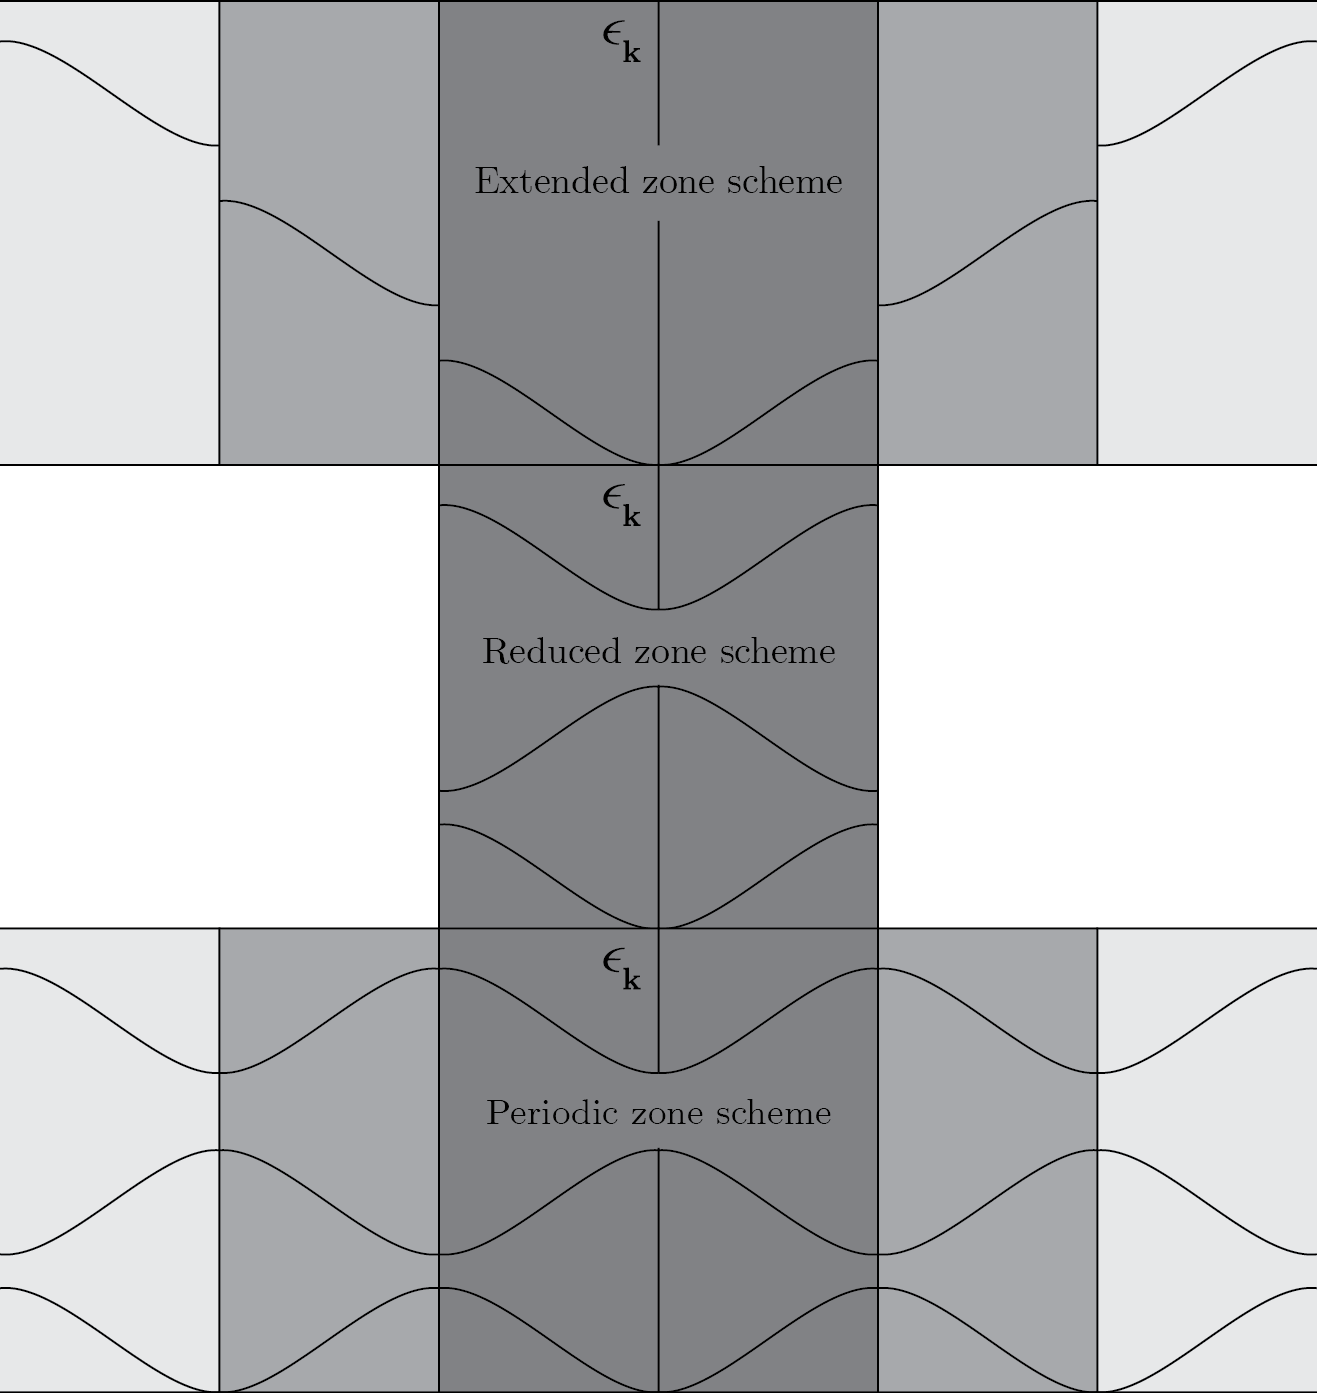
\includegraphics[width=0.6\textwidth]{\figurepath/dft/reduced.png} 
\caption{\label{dft:fig-reduced}The reduced zone scheme, derived from the extended 
zone scheme by mapping all bands to the first Brillouin zone. If we repeat the 
reduced zone scheme for the whole reciprocal space, we obtain the so-called 
periodic zone scheme. Taken from~\cite{Kittel2004}.} 
\end{figure} 
 
\subsection{Basis Set} \label{dft:sec-basis_set} 
 
In order to find the Kohn-Sham orbitals, the one electron wave functions are 
expanded in a certain basis set. Although in principle any basis set can be 
used, it is preferable to look for a set of basis functions that strikes a good balance between being  
\textit{efficient} and \textit{unbiased}. This means that the wave functions 
can be expanded in a relatively small number of basis functions and that the 
set is not tailored to suit a specific problem~\cite{Cottenier2013}. An 
example of a set of functions that are certainly unbiased are the plane waves $e^{i \mathbf{G}\cdot 
\mathbf{r}}$, where $\mathbf{G}$ is a reciprocal lattice vector. If we write 
$u_{n\mathbf{k}}(\mathbf{r})$ in Eq. (\ref{dft:eq-bloch}) as a linear combination of 
these basis functions, we find 
\begin{eqnarray} 
\phi_{n\mathbf{k}}(\mathbf{r}) &=& \left( \sum_{\mathbf{G}} 
c_{n\mathbf{k}}^{\mathbf{G}}e^{i\mathbf{G}\cdot \mathbf{r}} \right) 
e^{i\mathbf{k}\cdot \mathbf{r}} 
\\ \label{dft:eq-planewaves} &=& \sum_{\mathbf{G}} 
c_{n\mathbf{k}}^{\mathbf{G}}e^{i(\mathbf{G}+\mathbf{k})\cdot \mathbf{r}}. 
\end{eqnarray} 
 
If we want to find the coefficients $c_{n\mathbf{k}}^{\mathbf{G}}$, we have to 
solve the eigenvalue problem derived from the Kohn-Sham equations. This 
requires diagonalisation of the Hamiltionian matrix in the basis set. In 
principle, the basis set can be infinitely large, but for practical 
calculations we have to put a limit on the number of basis functions. This 
limit is defined by only including terms with a reciprocal lattice vector $G 
\leq G_{max}$, which is usually determined by considering the maximum energy: 
\begin{equation} \label{dft:eq-energy_cutoff}
E_{cut} = \frac{\hbar^2 G_{max}^2}{2m_e}. 
\end{equation} 
The \textit{cutoff energy} $E_{cut}$ is an input parameter for the 
calculations that determines how many plane waves are included in the basis 
set. In other words, increasing $E_{cut}$ improves the precision of the 
calculation, but results in a more difficult diagonalization procedure for the 
Hamiltonian.  

\phantomsection \label{dft:sec-gaussian}
For non-periodic problems, such as the anion-cation system described in Section~\ref{batteries:sec-landscape}, it is often more efficient to rely on a localized basis set. A popular example of such a basis set is the Gaussian basis set, often used in molecular calculations. Here, the basis set consists of functions with the following form~\cite{Hill2013}: 
\begin{equation}
\chi(\zeta, n, m, l; r, \theta, \phi) = N Y_{l,m}(\theta, \phi) r^{2n-2-l} e^{-\zeta r^2},
\end{equation}
where $\zeta$ is known as the exponent, $n$, $m$ and $l$ are the orbital quantum numbers, $N$ is a normalization constant and $Y_{l,m}(\theta, \phi)$ are the spherical harmonic functions. 
 
\subsection{Pseudopotentials} 
 
The efficiency of the plane wave basis set depends on 
how large $E_{cut}$ must be in order for Eq.~(\ref{dft:eq-planewaves}) to correctly describe the wave function $\phi (\mathbf{r})$. 
This, in turn, is connected with how much $\phi (\mathbf{r})$ varies in the 
region around $\mathbf{r}$~\cite{Kohanoff2006}. When looking at 
Fig.~\ref{dft:fig-pseudo}, we can see that the radial part of the electron 
orbitals varies the most near the nucleus of an atom, where the interaction is 
stronger. However, the region which is important for the chemical bonds lies 
further from the nucleus, and here the wave function is relatively smooth. In the 
interest of keeping the calculations manageable, it is desirable to replace 
the quickly oscillating wave function with a smoother version, which still has 
the same value as the actual wave function in the region of the chemical bond. 
 
\begin{figure}[ht]  
\captionsetup{width=0.8\textwidth} 
\centering 
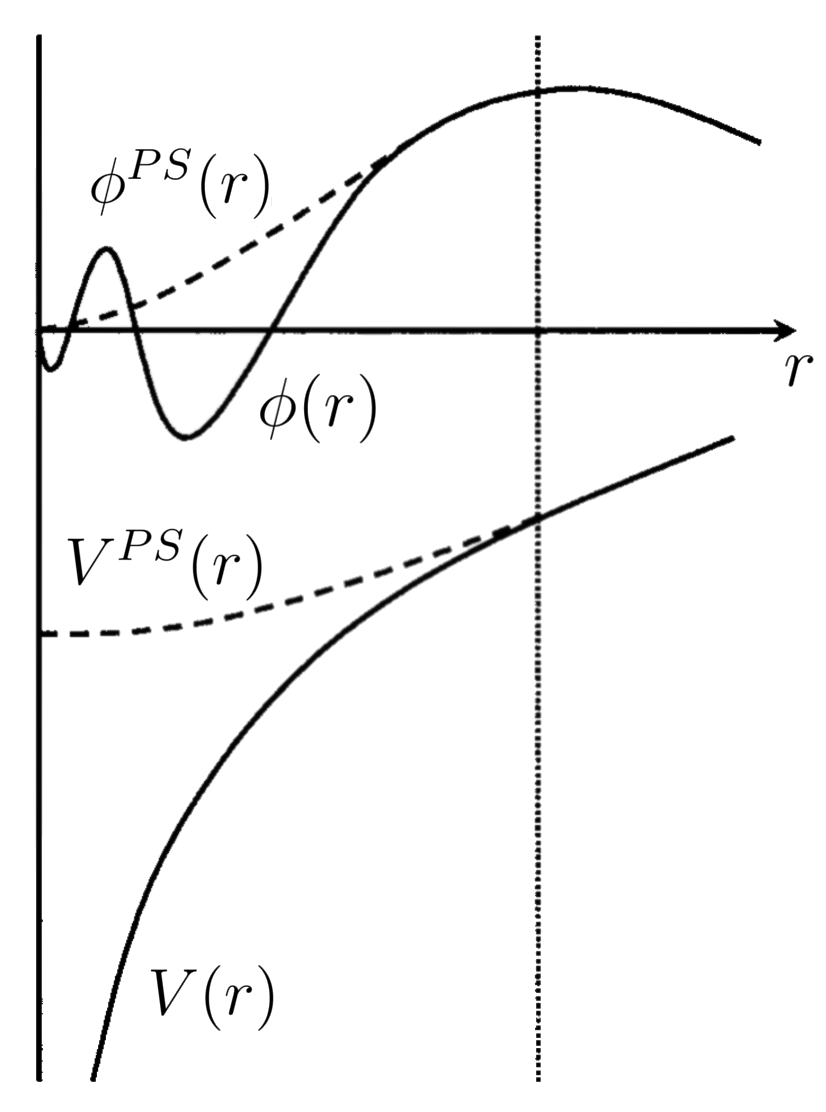
\includegraphics[width=0.35\textwidth]{\figurepath/dft/pseudopot.png} 
\caption{\label{dft:fig-pseudo} Schematic representation of the pseudopotential 
method. The true wave function (dashed curve) has several nodes, and is 
replaced by the smoothed version (full curve) after the introduction of the 
pseudopotential. Adapted from~\cite{Singh2006}.} 
\end{figure} 
 
We can achieve this goal by replacing the potential of the nuclei by a 
\textit{pseudopotential} (\gls{PP})~\cite{Phillips1959}. Firstly, we make a 
distinction between two types of electrons in the atom: the \textit{core} 
electrons are highly localized and are considered together with the nucleus, 
whereas the \textit{valence electrons} are responsible for the bonding and are 
treated explicitly. In this formalism, we can construct the true valence wave 
functions $\ket{\phi_v}$ by combining a smooth wave function 
$\ket{\tilde{\phi}_v}$ with a linear combination of the core electron wave 
functions $\ket{\phi_c}$~\cite{Kohanoff2006}: 
\begin{equation} \label{dft:eq-valence}
\ket{\phi_v} = \ket{\tilde{\phi}_v} + \sum_c \alpha_{vc} \ket{\phi_c},  
\end{equation} 
where $\alpha_{vc} = - \braket{\phi_c | \tilde{\phi}_v}$ in order to make the 
wave function $\ket{\phi_v}$ orthogonal to the core wave functions. In the 
case of \gls{DFT}, we need to solve the Kohn-Sham equations (Eq.~(\ref{dft:eq-KS})): 
\begin{equation}\label{dft:eq-KS2} 
\underbrace{\left[- \frac{1}{2} \Delta_{\mathbf{r}} + V_{eff}(\mathbf{r}) 
\right]}_{\hat{H}_{KS} } \ket{\phi_v} = \epsilon_v \ket{\phi_v}. 
\end{equation} 
Inserting $\ket{\phi_v}$ from Eq.~(\ref{dft:eq-valence}) into Eq. (\ref{dft:eq-KS2}), we find 
\begin{align*} 
&\hspace{0.5in}\hat{H}_{KS} \ket{\phi_v} = \epsilon_v \ket{\phi_v}  
\\ \Leftrightarrow &\hspace{0.5in} \hat{H}_{KS} \ket{\tilde{\phi}_v} + \sum_c 
\alpha_{vc} \epsilon_c \ket{\phi_c} = \epsilon_v \ket{\tilde{\phi}_v} +  
\sum_c \epsilon_v \alpha_{vc}  \ket{\phi_c} 
\\ \Leftrightarrow &\hspace{0.5in} \hat{H}_{KS} \ket{\tilde{\phi}_v} + \sum_c 
(\epsilon_c - \epsilon_v) \alpha_{vc}  \ket{\phi_c} = \epsilon_v 
\ket{\tilde{\phi}_v} 
\\ \Leftrightarrow &\hspace{0.5in} \left[ \hat{H}_{KS} + \sum_c (\epsilon_v - 
\epsilon_c) \ket{\phi_c} \bra{\phi_c} \right] \ket{\tilde{\phi}_v} = 
\epsilon_v \ket{\tilde{\phi}_v}. 
\end{align*} 
We define the pseudopotential $\hat{V}_{PP}(\mathbf{r})$ by adding the 
operator 
\begin{equation*} 
\sum_c (\epsilon_v - \epsilon_c) \ket{\phi_c} \bra{\phi_c} 
\end{equation*} 
to the effective Kohn-Sham potential: 
\begin{equation} 
\hat{V}_{PP}(\mathbf{r}) = V_{eff}(\mathbf{r}) + \sum_c (\epsilon_v - 
\epsilon_c) \ket{\phi_c} \bra{\phi_c}. 
\end{equation} 
The Kohn-Sham equations are now transformed into: 
\begin{equation} 
\left[- \frac{1}{2} \Delta_{\mathbf{r}} + \hat{V}_{PP}(\mathbf{r}) 
\right]\ket{\tilde{\phi}_v} = \epsilon_v \ket{\tilde{\phi}_v}, 
\end{equation} 
which is the single particle equation for the smooth part of the wave 
function. Finding accurate approximations for the pseudopotential operator is 
a scientific discipline in its own right, and there is a large variety of 
possible methods of constructing pseudopotentials. For an overview, we refer 
the reader to~\cite{Singh2006}. 
 
\subsection{Projector Augmented Waves} \label{dft:sec-PAW} 
 
The main drawback of the pseudopotential method is that all the information on 
the full electron wave function near the the nuclei is 
lost. A more general approach is the projector augmented 
wave (\gls{PAW}) method, which was first introduced by Bl\"ochl in 
1994~\cite{Blochl1994}. This method has similarities with the \gls{PP} approach, in 
the sense that it tries to replace the true all-electron (\gls{AE}) wave function 
with a smoother pseudo (\gls{PS}) wave function, that agrees with the true wave 
function in the bonding region. Here I present a brief discussion of the concept,
largely based on the excellent paper of Rostgaard~\cite{Rostgaard2009}.
 
We consider each nucleus to be enclosed by a spherical volume of radius $R_a$, 
called the \textit{augmentation} region $\Omega_{R_a}$, and define the 
remaining part of space as the \textit{interstitial} region. We are looking 
for a linear operator that transforms the computationally convenient \gls{PS} one 
electron wave functions $\ket{\tilde{\phi}}$ into the physically relevant \gls{AE}
one-electron wave functions $\ket{\phi}$: 
\begin{equation}\label{dft:eq-PAW} 
\ket{\phi} = \hat{\mathcal{T}} \ket{\tilde{\phi}}. 
\end{equation} 
Since we only want to modify the wave functions near the nuclei, we can write 
the transformation operator in the form 
\begin{equation} 
\hat{\mathcal{T}} = 1 + \sum_a \hat{\mathcal{T}}_{R_a}, 
\end{equation} 
where each operator $\hat{\mathcal{T}}_{R_a}$ is a null operator\footnote{A 
null operator is an operator $\hat{A}$ which reduces any state to 
zero:\begin{equation*}\hat{A}\ket{\alpha}=0\hspace{0.3in}\text{for any } 
\ket{\alpha}.\end{equation*}} outside the augmentation region of atom $a$. 
Inside each augmentation region $\Omega_{R_a}$, we expand the \gls{AE} wave function 
in partial waves $\ket{\varphi_i^a}$ and the \gls{PS} wave function in partial waves 
$\ket{\tilde{\varphi}_i^a}$: 
\begin{equation} 
\ket{\phi^a} = \sum_i c_i^a \ket{\varphi_i^a} \hspace{0.4in} 
\ket{\tilde{\phi}^a} = \sum_i \tilde{c}_i^a \ket{\tilde{\varphi}_i^a}, 
\end{equation} 
and require that the partial waves can be transformed using the same operator 
as the \gls{AE} and \gls{PS} wave function: 
\begin{equation}\label{dft:eq-transpartial} 
\forall a,i:\hspace{0.3in}\ket{\varphi_i^a} = \left( 1 + 
\hat{\mathcal{T}}_{R_a} \right) \ket{\tilde{\varphi}_i^a} \hspace{0.1in} 
\Leftrightarrow \hspace{0.1in} \hat{\mathcal{T}}_{R_a} 
\ket{\tilde{\varphi}_i^a} = \ket{\varphi_i^a} - \ket{\tilde{\varphi}_i^a}. 
\end{equation} 
This completely defines $\hat{\mathcal{T}}$ for a given set of partial waves 
$\varphi_i^a,\tilde{\varphi}_i^a$. Since we have 
\begin{equation} 
\sum_i c_i^a \ket{\varphi_i^a} = \ket{\phi^a} = \hat{\mathcal{T}} 
\ket{\tilde{\phi}^a} = \sum_i \tilde{c}_i^a \hat{\mathcal{T}} 
\ket{\tilde{\varphi}_i^a} = \sum_i \tilde{c}_i^a \ket{\varphi_i^a}, 
\end{equation} 
we can see that the coefficients for both expansions are the same ($c_i^a = 
\tilde{c}_i^a$). Also, because the operators $\hat{\mathcal{T}}_R$ are null 
operators outside their augmentation regions $\Omega_R$, we can derive from 
Eq.~(\ref{dft:eq-transpartial}) that the partial waves are the same in the 
interstitial region ($\ket{\varphi_i^a} = \ket{\tilde{\varphi}_i^a}$). 
 
Since we are looking for a linear transformation $\hat{\mathcal{T}}$, the 
coefficients $c_i^a$ have to be linear functionals of the \gls{PS} wave function: 
\begin{equation} 
c_i^a = \braket{\tilde{p}_i^a | \tilde{\phi}^a}. 
\end{equation} 
The $\bra{\tilde{p}_i^a}$ are called the \textit{projector functions}. Inside 
each augmentation region, the one-center expansion of the \gls{PS} wave function is 
equal to itself: 
\begin{equation} 
\sum_i \ket{\tilde{\varphi}_i^a}\braket{\tilde{p}_i^a | \tilde{\phi}^a} = 
\ket{\tilde{\phi}^a},\hspace{0.1in}\text{from which} \hspace{0.1in} \sum_i 
\ket{\tilde{\varphi}_i^a}\bra{\tilde{p}_i^a} = 1.  
\end{equation} 
Using this completeness relation in combination with 
Eq.~(\ref{dft:eq-transpartial}), we find the following expression for the 
transformation operator in $\Omega_{R_a}$: 
\begin{equation} 
\hat{\mathcal{T}}_{R_a} = \sum_i \hat{\mathcal{T}}_{R_a} 
\ket{\tilde{\varphi}_i^a}\bra{\tilde{p}_i^a} = \sum_i(\ket{\varphi_i^a} - 
\ket{\tilde{\varphi}_i^a})\bra{\tilde{p}_i^a}, 
\end{equation} 
from which we can conclude that the total transformation operator is equal to: 
\begin{equation}\label{dft:eq-transform} 
\hat{\mathcal{T}} = 1 + \sum_a \sum_i(\ket{\varphi_i^a} - 
\ket{\tilde{\varphi}_i^a})\bra{\tilde{p}_i^a}. 
\end{equation} 
 
Using the \gls{PAW} method changes the regular Kohn-Sham equations 
(Eq.~(\ref{dft:eq-KS})) for an \gls{AE} wave function $\ket{\phi}$ with energy 
$\epsilon$ to an eigenvalue equation for the \gls{PS} wave function: 
\begin{equation}\label{dft:eq-KSPAW} 
\hat{\mathcal{T}}^\dagger \hat{H}_{KS} \hat{\mathcal{T}} \ket{\tilde{\phi}} = 
\epsilon \hat{\mathcal{T}}^\dagger \hat{\mathcal{T}} \ket{\tilde{\phi}}. 
\end{equation} 
After solving Eq.~(\ref{dft:eq-KSPAW}), we can construct the \gls{AE} wave function by 
using Eq.~(\ref{dft:eq-PAW}) and Eq.~(\ref{dft:eq-transform}): 
\begin{equation} 
\ket{\phi} = \hat{\mathcal{T}} \ket{\tilde{\phi}} = \left(1 + \sum_a 
\hat{\mathcal{T}}_{R_a}\right) \ket{\tilde{\phi}}= \ket{\tilde{\phi}} + \sum_a 
\sum_i(\ket{\varphi_i^a} - \ket{\tilde{\varphi}_i^a})\braket{\tilde{p}_i^a | 
\tilde{\phi}}, 
\end{equation} 
which in position space becomes 
\begin{eqnarray} 
\phi(\mathbf{r}) = \braket{\mathbf{r} | \phi} &=& \braket{\mathbf{r} 
|\tilde{\phi}} + \sum_a \sum_i(\braket{\mathbf{r} | \varphi_i^a} - 
\braket{\mathbf{r} | \tilde{\varphi}_i^a})\braket{\tilde{p}_i^a | 
\tilde{\phi}} 
\\&=& \tilde{\phi}(\mathbf{r}) + \sum_a \sum_i(\varphi_i^a(\mathbf{r}) - 
\tilde{\varphi}_i^a (\mathbf{r}))\braket{\tilde{p}_i^a | \tilde{\phi}}. 
\end{eqnarray} 
 
The \gls{PAW} method is implemented using large data sets for each element. Such a 
data set governs exactly how the \gls{PAW} transformation works for each atomic 
site. One has a large degree of freedom when generating data sets for \gls{PAW} 
transformations, which are determined by the partial waves 
$\varphi_i^a,\tilde{\varphi}_i^a$ and the projector augmented functions 
$\tilde{p}_i^a(\mathbf{r}) = \braket{\mathbf{r} |\tilde{p}_i^a}$. For more 
information, we refer the reader to~\cite{Rostgaard2009}. 
 
\subsection{K-point Mesh} \label{dft:sec-kpoints} 
 
For an infinite crystal lattice, $\mathbf{k}$ is a continuous variable, which 
means that the calculation of many properties of the system requires an 
integration over the first Brillouin zone (\gls{BZ}). When doing numerical 
calculations, however, this is not practically possible. Instead, we make a 
selection of $\mathbf{k}$ points over which we sum the function in order to 
approximate the integration: 
\begin{equation} \label{dft:eq-BZint} 
\frac{1}{\Omega_{BZ}}\int_{BZ} f(\mathbf{k}) d\mathbf{k} \simeq 
\frac{1}{N_\mathbf{k}} \sum_\mathbf{k} f(\mathbf{k}), 
\end{equation} 
where $N_\mathbf{k}$ is the number of chosen $\mathbf{k}$-points. This set of 
reciprocal points is commonly referred to as the~\textit{k-point mesh}. 
Figure~\ref{dft:fig-k_mesh} presents an example of a $\mathbf{k}$-mesh for the \gls{BZ} 
of the two dimensional square lattice. It also shows the irreducible 
Brillouin zone \gls{IBZ}, which is the smallest possible subspace of the 
Brillouin zone that can be used to construct the whole \gls{BZ} by the symmetry 
operations of the crystal's space group.  
 
As a result of the crystal's symmetry, which is determined by the lattice and 
atom positions, some of the $\mathbf{k}$-points are equivalent. This means 
that they can be mapped on each other using the symmetry operations of the 
space group. For equivalent $\mathbf{k}$-points, the value of the function 
$f(\mathbf{k})$ provides the same contribution to the sum in 
Eq.~(\ref{dft:eq-BZint}). It is therefore convenient to only calculate the value 
of $f(\mathbf{k})$ for the \textit{irreducible} $\mathbf{k}$-points of the 
$\mathbf{k}$-mesh. This is the smallest set of inequivalent 
$\mathbf{k}$-points of the $\mathbf{k}$-mesh from which the whole 
$\mathbf{k}$-mesh can be retrieved through a combination of symmetry 
operations. In case the $\mathbf{k}$-mesh has the same symmetry as the space 
group, the irreducible $\mathbf{k}$-points are found in the \gls{IBZ}. 
 
If $\{\mathbf{k}_i\}$ is the set of irreducible $\mathbf{k}$-points, the sum 
in Eq.~(\ref{dft:eq-BZint}) can be expressed as: 
\begin{equation} 
\frac{1}{N_\mathbf{k}} \sum_\mathbf{k} f(\mathbf{k}) =  \sum_{\mathbf{k}_i} 
w_{\mathbf{k}_i} f(\mathbf{k}_i), 
\end{equation} 
where $w_{\mathbf{k}_i}$ is the weight of $\mathbf{k}_i$. The weight of an 
irreducible $\mathbf{k}$-point is defined as the number of equivalent 
$\mathbf{k}$-points of the total mesh that correspond to this 
$\mathbf{k}$-point, divided by the total number of $\mathbf{k}$-points in the 
mesh (Fig.~\ref{dft:fig-k_mesh}). 
 
\begin{figure}[ht]  
\centering 
\begin{tikzpicture}[scale=1.3, font=\large, >=latex, auto, thick, 
kcircle/.style={draw, circle, color=red, minimum size = 0.4cm} 
] 
    % Reciprocal axes 
    \draw [->] (0, 0) node [left] {$\Gamma$} -- (3, 0) node [below] 
{$\mathbf{b}_1$}; 
    \draw [->] (0, 0) -- (0, 3) node [left] {$\mathbf{b}_2$}; 
     
    % Brillouin zone 
    \draw (-2, -2) rectangle (2, 2); 
    \draw [dashed] (0, 0) -- (2, 2); 
    \path [fill=black, fill opacity=0.3] (0, 0) -- (2, 2) -- (2, 0) -- cycle; 
     
    % k-points 
    \foreach \x in {-1.5, -0.5, ..., 1.5} 
        \foreach \y in {-1.5, -0.5, ..., 1.5} 
            \draw[fill=blue, color=blue] (\x,\y) circle (0.1cm); 
     
    \node (k1) at (0.5, 0.5) [kcircle] {}; 
    \node (k2) at (1.5, 1.5) [kcircle] {}; 
    \node (k3) at (1.5, 0.5) [kcircle] {}; 
     
    % Annotation 
    \node (k1_anno) at (1.3, 2.7) {$\mathbf{k}_1$}; 
    \draw [->, thin] (k1_anno)  -- (k1); 
    \node (k2_anno) at (2, 2.7) {$\mathbf{k}_2$}; 
    \draw [->, thin] (k2_anno)  -- (k2); 
    \node (k3_anno) at (2.7, 2.7) {$\mathbf{k}_3$}; 
    \draw [->, thin] (k3_anno)  -- (k3); 
     
    \node (bz) at (3, -1) {BZ}; 
    \draw (1.9, -1) -- (bz); 
    \node (ibz) at (3, 1) {IBZ}; 
    \draw (1.9, 1) -- (ibz); 
     
\end{tikzpicture} 
\caption{\label{dft:fig-k_mesh}Illustration of the $\mathbf{k}$-point mesh for a 
two dimensional square lattice. The irreducible \textbf{k}-points are 
highlighted by a red circle. The weights for the three irreducible 
$\mathbf{k}$-points are: $w_{\mathbf{k}_1} = \frac{1}{4}$ , $w_{\mathbf{k}_2} 
= \frac{1}{4}$ , $w_{\mathbf{k}_3} = \frac{1}{2}$.} 
\end{figure} 

\phantomsection \label{dft:sec-monkhorst}
A common collection of $\mathbf{k}$-points used in \gls{DFT} calculations is the 
Monkhorst-Pack mesh~\cite{Monkhorst1976}, which is an equidistant grid defined 
as: 
\begin{equation} 
\mathbf{k}(n_1,n_2,n_3) = \sum_{i=1}^{3} \frac{2n_i - N_i - 1}{2N_i} 
\mathbf{b}_i, 
\end{equation} 
where the $\mathbf{b}_i$ are the basis vectors of the reciprocal lattice and the $n_i$ run 
from $1$ to $N_i$. After the Monkhorst-Pack mesh is created, it is usually 
shifted in order to make it centered around the $\Gamma$-point. This way we 
can increase the symmetry of the $\mathbf{k}$-mesh, which lowers the amount of 
irreducible $\mathbf{k}$-points, making our calculations less cumbersome. This 
is illustrated for the two dimensional square lattice in 
Figure~\ref{dft:fig-k_mesh}. 
 
\section{Linear Response Theory} \label{dft:sec-linear} 

Many important properties of materials are based on its response to external 
electric fields. Optical properties, such as the absorption coefficient used 
for the calculation of the selection metric described in 
Section~\ref{slme:sec-SLME}, depend on the dielectric response of the material 
in the long-wavelength limit. So does the electron energy loss function, used in 
Section~\ref{quotas:sec-plasmons} to introduce plasmonic excitations to our 
model of secondary electron emission. In this section I present a shortened 
derivation of the expression used to calculate the dielectric tensor, largely 
based on the excellent thesis of Judith Harl~\cite{Harl2008}.

\subsection{Response Function} 

The dielectric tensor expresses the optical properties of the material, which 
depend on the response of the material to external electric fields. In linear 
response theory, the response of the material to an external electric field is 
described by the response function $\chi(\mathbf{r},\mathbf{r}', t - t')$, 
which determines the change in density $\delta \rho$ at ($\mathbf{r},t$) if the 
external potential undergoes a small change $\delta v_{exp}$ at 
($\mathbf{r}',t'$)~\cite{Harl2008}: 
\begin{equation}\label{dft:eq-response} 
\delta \rho (\mathbf{r},t) = \int dt' \int d\mathbf{r}' 
\chi(\mathbf{r},\mathbf{r}', t - t') \delta v_{exp} (\mathbf{r}',t'). 
\end{equation} 
Within the time-dependent Kohn-Sham formalism, the response function 
$\chi^{KS}(\mathbf{r},\mathbf{r}, t - t')$ describes the change in density in 
response to a small change in the effective potential $\delta 
V_{eff}(\mathbf{r},t)$: 
\begin{equation}\label{dft:eq-KSresponse} 
\delta \rho (\mathbf{r},t) = \int dt' \int d\mathbf{r}' 
\chi^{KS}(\mathbf{r},\mathbf{r}', t - t') \delta V_{eff} (\mathbf{r}',t'). 
\end{equation} 
 
Following the derivation of Pines and Nozi\`eres~\cite{Nozieres1994}, it is 
possible to use perturbation theory to write the Kohn-Sham response function 
in frequency space as 
\begin{equation}\label{dft:eq-pines} 
\chi^{KS}(\mathbf{r},\mathbf{r}', \omega) = - \sum_{i,j} f_i \left(1 - f_j\right) \left( 
\frac{\phi_j^*(\mathbf{r'})\phi_i(\mathbf{r'})\phi_i^*(\mathbf{r})\phi_j(\mathbf{r})}{\epsilon_j 
- \epsilon_i - \check{\omega}} + 
\frac{\phi_i^*(\mathbf{r'})\phi_j(\mathbf{r'})\phi_j^*(\mathbf{r})\phi_i(\mathbf{r})}{\epsilon_j 
- \epsilon_i + \check{\omega}} \right), 
\end{equation} 
\\ 
where $\phi_i(\mathbf{r})$ are the \gls{KS} orbitals of the time-independent 
problem~(Eqs.~(\ref{dft:eq-KS})), and $\check{\omega} = \omega + i \eta$ is a 
complex deviation from the angular frequency $\omega$, introduced in the 
perturbation calculation. The occupancies $f_i$ are included in Eq~(\ref{dft:eq-pines}) in 
such a way that the coefficient in the sum is equal to 1 only when the 
i$^{th}$ orbital is occupied and the j$^{th}$ orbital is unoccupied. Next, we 
use the periodicity of the crystal and take the Fourier transform of 
Eq.~(\ref{dft:eq-pines}). Because the real space response function is invariant 
with respect to a shift by a lattice vector \textbf{R}:  
\begin{equation} 
\chi^{KS}(\mathbf{r} + \mathbf{R},\mathbf{r}' + \mathbf{R}, \omega) = 
\chi^{KS}(\mathbf{r},\mathbf{r}', \omega), 
\end{equation} 
it is possible to demonstrate that the Fourier transform 
$\chi^{KS}(\mathbf{g},\mathbf{g}',\omega)$ is only nonzero when the two wave 
vectors $\mathbf{g}$ and $\mathbf{g}'$ differ by a reciprocal lattice vector: 
$\mathbf{g} = \mathbf{g}' + \mathbf{G}''$. Since we can write $\mathbf{g}'$ as 
the sum of a vector in the first Brillouin zone $\mathbf{q}$ and a reciprocal 
lattice vector $\mathbf{G}'$, we can do the same for $\mathbf{g} = \mathbf{g} 
+ \mathbf{G}'' = \mathbf{q} + \mathbf{G} + \mathbf{G}'' = \mathbf{q} + 
\mathbf{G}'$. This can be used to express the momentum space response function 
as $\chi_{\mathbf{G},\mathbf{G}'}^{KS}(\mathbf{q},\omega)$, where $\mathbf{G}$ 
and $\mathbf{G}'$ are two reciprocal lattice vectors and $\mathbf{q}$ is a 
reciprocal vector lying in the first Brillouin zone. Next, we use the Bloch 
theorem to write the states as we did in Section~\ref{dft:sec-bloch}. The 
combination of all these considerations allows us to formulate the response 
function in momentum space: 
\begin{equation} 
\begin{aligned} 
\chi_{\mathbf{G},\mathbf{G}'}^{KS}(\mathbf{q},\omega) = - \frac{1}{V} 
\sum_{n\mathbf{k},m\mathbf{k}'} f_{n\mathbf{k}} (1 - f_{m\mathbf{k}'}) 
\left( \frac{\braket{\phi_{m\mathbf{k}'} | 
e^{i(\mathbf{q}+\mathbf{G})\cdot\mathbf{r}} 
|\phi_{n\mathbf{k}}}\braket{\phi_{n\mathbf{k}} | 
e^{-i(\mathbf{q}+\mathbf{G}')\cdot\mathbf{r}'} 
|\phi_{m\mathbf{k}'}}}{\epsilon_{m\mathbf{k}'} - \epsilon_{n\mathbf{k}} - 
\check{\omega}}\right. \\ \left. + \frac{\braket{\phi_{n\mathbf{k}} | 
e^{i(\mathbf{q}+\mathbf{G})\cdot\mathbf{r}} 
|\phi_{m\mathbf{k}'}}\braket{\phi_{m\mathbf{k}'} | 
e^{-i(\mathbf{q}+\mathbf{G}')\cdot\mathbf{r}'} 
|\phi_{n\mathbf{k}}}}{\epsilon_{m\mathbf{k}'} - \epsilon_{n\mathbf{k}} + 
\check{\omega}}\right). 
\end{aligned} 
\end{equation} 
This can alternatively be written as~\cite{Harl2008} 
\begin{equation} \label{dft:eq-Fresponse} 
\begin{aligned} 
\chi_{\mathbf{G},\mathbf{G}'}^{KS}(\mathbf{q},\omega) = - \frac{1}{V} 
\sum_{n,m ; \mathbf{k}} f_{n\mathbf{k}} \braket{u_{m\mathbf{k+q}} | 
e^{i\mathbf{G}\cdot\mathbf{r}} | u_{n\mathbf{k}}} \braket{u_{n\mathbf{k}} | 
e^{-i\mathbf{G}'\cdot\mathbf{r}'} | u_{m\mathbf{k+q}}}\\ \cdot \left( 
\frac{1}{\epsilon_{m\mathbf{k+q}} - \epsilon_{n\mathbf{k}} - \check{\omega}} + 
\frac{1}{\epsilon_{m\mathbf{k+q}} - \epsilon_{n\mathbf{k}} + 
\check{\omega}}\right), 
\end{aligned} 
\vspace{0.2in} 
\end{equation} 
where 
\begin{equation} 
\braket{u_{m\mathbf{k+q}} | e^{i\mathbf{G}\cdot\mathbf{r}} | u_{n\mathbf{k}}} 
\equiv \int_V d\mathbf{r} \hspace{0.05in} u_{m\mathbf{k+q}}^*(\mathbf{r}) 
e^{i\mathbf{G}\cdot\mathbf{r}} u_{n\mathbf{k}}(\mathbf{r}) 
\end{equation} 
are integrals over the volume $V$ of the unit cell. 
 
\subsection{Dielectric Tensor} \label{dft:sec-dielectric} 
 
In order to derive the microscopic dielectric function, we use the 
\textit{random phase approximation} (RPA), which connects the dielectric 
function to the Kohn-Sham response function as follows~\cite{Harl2008}: 
\begin{equation}\label{dft:eq-micdiel} 
\varepsilon_{\mathbf{G},\mathbf{G}'}(\mathbf{q},\omega) = 
\delta_{\mathbf{G},\mathbf{G}'} - \frac{4 \pi}{|\mathbf{G} + \mathbf{q}| 
|\mathbf{G}' + \mathbf{q}|} 
\chi_{\mathbf{G},\mathbf{G}'}^{KS}(\mathbf{q},\omega), 
\end{equation} 
where $\delta_{\mathbf{G},\mathbf{G}'}$ is the Kronecker delta. However, for
wavelengths that are much larger than the periodicity of the system, we are 
interested in macroscopic averages of the dielectric response, not the rapid 
fluctuations at the microscopic level. Following the derivation of 
Harl~\cite{Harl2008}, the relation between the microscopic and macroscopic 
dielectric function is
\begin{equation}
\varepsilon_{\text{mac}}(\mathbf{q}, \omega) = 
(\varepsilon_{0,0}^{-1}(\mathbf{q}, \omega))^{-1}.
\end{equation}
When we ignore local field effects, the off-diagonal elements of the 
microscopic dielectric tensor are neglected, and the macroscopic dielectric 
function can be approximated as: 
\begin{equation} 
\varepsilon_{\text{mac}}(\mathbf{q}, \omega) = \varepsilon_{0,0}(\mathbf{q}, \omega) 
\underset{(\ref{dft:eq-micdiel})}{=} 1 - \frac{4 
\pi}{q^2} \chi_{0,0}^{KS}(\mathbf{q},\omega). 
\end{equation} 
For optical properties, we consider the long-wavelength limit ($\mathbf{q} 
\rightarrow 0$) of the macroscopic dielectric function, also written as 
$\varepsilon_\infty (\mathbf{\hat{q}}, \omega)$:
\begin{equation}
\varepsilon_\infty (\mathbf{\hat{q}}, \omega) = \lim_{q \rightarrow 0} 
\varepsilon_{\text{mac}}(\mathbf{q}, \omega) =  1 - \lim_{q \rightarrow 0} 
\frac{4 \pi}{q^2} \chi_{0,0}^{KS}(\mathbf{q},\omega). 
\end{equation}

Using these approximations in combination with Eq.~(\ref{dft:eq-Fresponse}) allows 
us to evaluate the imaginary part of the macroscopic dielectric function 
$\varepsilon_\infty(\mathbf{\hat{q}},\omega) = 
\varepsilon_{\infty}^{(1)}(\mathbf{\hat{q}},\omega) + 
i\varepsilon_{\infty}^{(2)}(\mathbf{\hat{q}},\omega)$~\cite{Harl2008}: 
 \begin{equation}\label{dft:eq-imdiel} 
\varepsilon_{\infty}^{(2)}(\mathbf{\hat{q}},\omega) = \frac{4\pi}{V} \lim_{q 
\rightarrow 0} \frac{1}{q^2} \sum_{n,m,\mathbf{k}} f_{n\mathbf{k}} | 
\braket{u_{m\mathbf{k}+\mathbf{q}}|u_{n\mathbf{k}}} |^2 \cdot 
[\delta(\epsilon_{m\mathbf{k}}-\epsilon_{n\mathbf{k}}-\omega) - 
\delta(\epsilon_{m\mathbf{k}}-\epsilon_{n\mathbf{k}}+\omega)]. 
\end{equation} 
We introduce the macroscopic dielectric tensor by setting: 
\begin{equation} 
\varepsilon_{\infty}^{(2)}(\mathbf{\hat{q}},\omega) = \sum_{\alpha,\beta} 
\mathbf{\hat{q}}_\alpha \varepsilon_{\alpha \beta}^{(2)} (\omega) 
\mathbf{\hat{q}}_\beta. 
\end{equation} 
The imaginary part of the dielectric tensor is then calculated as: 
\begin{equation} \label{dft:eq-imdiel} 
\varepsilon_{\alpha \beta}^{(2)} (\omega) = \frac{4\pi}{V} \lim_{q 
\rightarrow 0} \frac{1}{q^2} \sum_{n,m;\mathbf{k}} f_{n\mathbf{k}} 
\braket{u_{m\mathbf{k}+q\mathbf{e}_\alpha}|u_{n\mathbf{k}}} 
\braket{u_{n\mathbf{k}}|u_{m\mathbf{k}+q\mathbf{e}_\beta}} \cdot 
[\delta(\epsilon_{m\mathbf{k}}-\epsilon_{n\mathbf{k}}-\omega) - 
\delta(\epsilon_{m\mathbf{k}}-\epsilon_{n\mathbf{k}}+\omega)], 
\end{equation} 
whereas the real part is found using the Kramers-Kronig transformation: 
\begin{equation} \label{dft:eq-kramers}
\varepsilon_{\alpha \beta}^{(1)} (\omega) = 1 + \frac{2}{\pi} \mathcal{P} 
\int_0^\infty \frac{\varepsilon_{\alpha \beta}^{(2)} 
(\omega')\omega'}{(\omega')^2 - \omega^2}d\omega', 
\end{equation} 
where $\mathcal{P}$ is the Cauchy Principal value~\cite{Gogolin2014}.  
 
I finish this section with a couple of notes. First, by introducing the 
\textbf{k}-mesh in Section~\ref{dft:sec-kpoints}, we can restrict the 
summation in Eq.~(\ref{dft:eq-imdiel}) to the irreducible \textbf{k}-points: 
\begin{align*} 
\varepsilon_{\alpha \beta}^{(2)} (\omega) = \frac{4\pi}{V} \lim_{q 
\rightarrow 0} \frac{1}{q^2} \sum_{n,m;\mathbf{k}_i}  f_{n\mathbf{k}_i} w_{\mathbf{k}_i} 
\braket{u_{m\mathbf{k}_i+q\mathbf{e}_\alpha}|u_{n\mathbf{k}_i}} 
\braket{u_{n\mathbf{k}_i}|u_{m\mathbf{k}_i+q\mathbf{e}_\beta}} \\  
\cdot [\delta(\epsilon_{m\mathbf{k}_i}-\epsilon_{n\mathbf{k}_i}-\omega) - 
\delta(\epsilon_{m\mathbf{k}_i}-\epsilon_{n\mathbf{k}_i}+\omega)], 
\end{align*} 
where $\mathbf{k}_i$ are the irreducible \textbf{k}-points with corresponding 
weights $w_{\mathbf{k}_i}$. Second, for semiconductors we can only consider 
interband transitions ($n \neq m$) between the valence and conduction band in the 
calculation of the dielectric tensor. Moreover, in this case the valence bands 
are fully occupied ($f_{n\mathbf{k}} = 2$), simplifying the expression 
further: 
\begin{equation} 
\varepsilon_{\alpha \beta}^{(2)} (\omega) = \frac{4\pi}{V} \lim_{q 
\rightarrow 0} \frac{1}{q^2} \sum_{c,v,\mathbf{k}_i} 2 w_{\mathbf{k}_i} \ 
\braket{u_{c\mathbf{k}_i+q\mathbf{e}_\alpha}|u_{v\mathbf{k}_i}} 
\braket{u_{v\mathbf{k}_i}|u_{c\mathbf{k}_i+q\mathbf{e}_\beta}} \cdot 
\delta(\epsilon_{c\mathbf{k}_i}-\epsilon_{v\mathbf{k}_i}-\omega)), 
\end{equation} 
where $c$ and $v$ denote the conduction and valence orbitals. 
 
Finally, we note that for each frequency $\omega$ it is possible to 
diagonalize the dielectric tensor. If we write the diagonal components as 
$\varepsilon_{11}(\omega) = \varepsilon_{x}(\omega)$, 
$\varepsilon_{22}(\omega) = \varepsilon_{y}(\omega)$ and 
$\varepsilon_{33}(\omega) = \varepsilon_{z}(\omega)$, we can calculate the 
complex index of refraction from the diagonal components of the diagonalized dielectric 
tensor as: 
\begin{equation} 
(n_c)_{\alpha}(\omega) = \sqrt{\varepsilon_{\alpha}(\omega)} \hspace{0.6in} 
\alpha = x,y,z. 
\end{equation} 
Using this relation, we can find the real index of refraction and extinction 
coefficient with the rules for taking the square root of a complex number: 
\begin{equation}\label{dft:eq-refindex} 
\begin{aligned} 
n_\alpha(\omega) = \sqrt{\frac{| \varepsilon_\alpha (\omega) | + 
\varepsilon_\alpha^{(1)}(\omega)}{2}} \\ 
k_\alpha(\omega) = \sqrt{\frac{| \varepsilon_\alpha (\omega) | - 
\varepsilon_\alpha^{(1)}(\omega)}{2}} 
\end{aligned}\hspace{0.6in} \alpha = x,y,z. 
\end{equation} 

\subsection{Drude model} \label{dft:sec-drude}

For metals, bands can be partially occupied, which means that we have to consider 
intraband transitions, i.e. where $n=m$ in the expressions of the previous section. 
In the long-wavelength limit, the intraband part of the dielectric tensor is 
included using the Drude model~\cite{Harl2008}:
\begin{equation}
\varepsilon_{\alpha\beta}^{(2), intra} (\omega) = \frac{\gamma\omega^2_{\alpha\beta}}{\omega
(\omega^2 + \gamma^2)},
\end{equation}
where $\gamma$ is the damping parameter. The so-called intraband plasma frequency 
(squared) $\omega^2_{\alpha\beta}$ is calculated from first-principles using the 
expression~\cite{Harl2008}:
\begin{equation}
\omega^2_{\alpha\beta} = \frac{4 \pi}{V} \sum_{n, \mathbf{k}} \frac{\partial 
f_{n\mathbf{k}}}{\partial \epsilon_{n\mathbf{k}}} \left(\mathbf{e}_\alpha \frac{\partial 
\epsilon_{n\mathbf{k}}}{\partial \mathbf{k}}\right) \left(\mathbf{e}_\beta \frac{\partial 
\epsilon_{n\mathbf{k}}}{\partial \mathbf{k}}\right).
\end{equation}
The imaginary part of the total dielectric tensor is the sum of the inter- and 
intraband contributions:
\begin{equation}
\varepsilon_{\alpha\beta}^{(2)} (\omega)  = \varepsilon_{\alpha\beta}^{(2), inter} 
(\omega) + \varepsilon_{\alpha\beta}^{(2), intra} (\omega),
\end{equation}
where the interband part is calculated via Eq.~(\ref{dft:eq-imdiel}). The real part 
is once again obtained via the Kramers-Kronig relationship (Eq.~(\ref{dft:eq-kramers})).

\section{Transition state theory}\label{dft:sec-transition} 

When considering a transition between two different states of a system, a 
first property of interest is the difference in energy $\Delta E$ between the 
final and initial state of the system, also referred to as the \textit{reaction energy}. For the comparison of the chalcopyrite 
and CuAu phases in Section~\ref{slme:sec-CuAu}, for example, comparing the formation energy 
of both structures can help us understand the likelihood of each phase being 
present after synthesis. In the case of the O-O dimerization in 
Section~\ref{batteries:sec-dimer}, the difference in energy between the 
initial and final state provides information on whether the formation 
of a specific dimer stabilizes the structure. 
 
\begin{figure}[ht] 
\centering
\begin{tikzpicture}[scale=2, thick, >=latex, auto] 
 
    % Initial and final state 
    \node (A) [inner sep=3pt] at (0, 0) {\Large A}; 
    \node (B) [inner sep=3pt] at (3.5, -1) {\Large B}; 
     
    % The barrier line 
    \draw (A) to[out=0, in=180] (0.7, 0); 
    \draw (0.7, 0) parabola (1.5, 1); 
    \draw (1.5, 1) to[out=70, in=180] (1.6, 1.1); 
    \draw (1.6, 1.1) to[out=0, in=110] (1.7, 1); 
    \draw (1.7, 1) parabola[bend at end] (3, -1); 
    \draw (3, -1) to[out=0, in=180] (B); 
     
    % The axes 
    \draw [->] (-0.4, -1.4) to node [above left=2em and 0em, rotate=90] 
{Energy} (-0.4, 1.7); 
    \draw [->] (-0.4, -1.4) to node [below] {Reaction Coordinate} ( (4, -1.4); 
     
    % Annotation 
    \draw [dashed] (0.2, 1.1) -- (1.6, 1.1); 
    \draw [<->] (0.4, 0) to node {$E_a$} (0.4, 1.1); 
     
    \draw [dashed] (0.6, -1) -- (3, -1); 
    \draw [<->] (0.7, 0) to node {$\Delta E$} (0.7, -1); 
     
\end{tikzpicture}  
\caption{\label{dft:fig-transition}Schematic of a transition from state A to state 
B.} 
\end{figure} 
 
However, often we are also interested in the kinetics of the transition, i.e. the 
rate at which a reaction will occur. One way of investigating this is by 
performing \textit{ab initio} molecular dynamics (AIMD) calculations. Unfortunately, 
for many reactions performing \gls{AIMD} simulations over a sufficiently long time 
scale to obtain relevant statistics is far too computationally demanding. A 
popular alternative for studying the kinetics is by obtaining the kinetic barrier, 
also known as the activation energy $E_a$, directly  
by determining the minimum energy path for the 
transition. Figure~\ref{dft:fig-transition} shows a schematic of the energy 
barrier of a transition. 
 
\subsection{Nudged elastic band method} \label{dft:sec-neb} 
 
A well established method for finding the minimum energy path between the 
initial and final state of the system is the nudged elastic band (\gls{NEB}) 
method~\cite{Jonsson1998, Henkelman2000}. In this technique, a path is 
constructed by considering a number of images in between the initial and final 
state, usually obtained by linearly interpolating the atomic positions of the initial and final 
structures. These images are then connected via fictitious springs in order to keep 
them spread somewhat evenly along the path, as simply optimizing the geometry 
of the images would revert them to either the initial or final state. This 
connected system is then optimized until the total force, i.e. a suitably 
chosen combination of the spring force and the \textit{true} force, is zero 
for each atom of each image.

\begin{figure}[ht] 
\centering
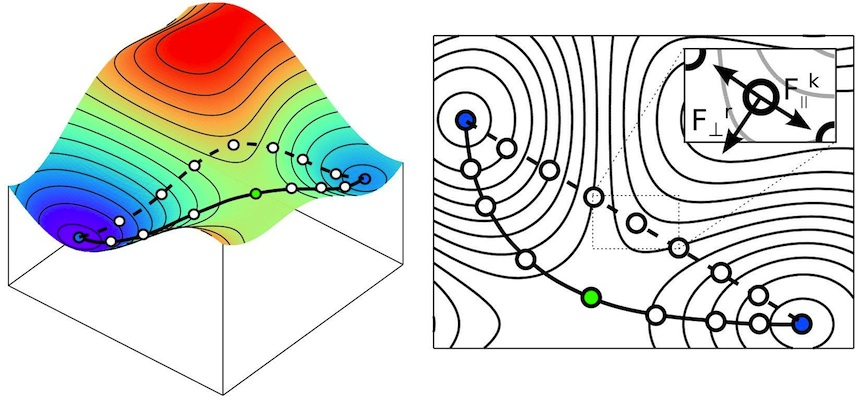
\includegraphics[width=0.8\textwidth]{figures/DFT/neb.jpg} 
\caption{\label{dft:fig-neb} Nudged elastic band method. Taken from~\cite{RheoMan2019}.} 
\end{figure} 

Write the $N + 1$ images as $\left[ \mathbf{R}_0,  \mathbf{R}_1,  
\mathbf{R}_2, ...,  \mathbf{R}_N  \right]$, where $ \mathbf{R}_0$ and $ 
\mathbf{R}_N$ are the coordinates of the initial and final state, respectively. The basic idea of 
the \gls{NEB} method is that the total force acting on an image is the sum of the 
spring force along the local tangent and the perpendicular part of the true 
force, i.e. the force on the image produced by the energy landscape: 
\begin{equation}\label{dft:eq-neb_force} 
\mathbf{F}_i = \mathbf{F}_i^s|_\parallel - \nabla E(\mathbf{R}_i)|_\perp.
\end{equation} 
The perpendicular part of the true force is calculated from the total true force and the 
projection on the local tangent $\boldsymbol{\hat{\tau}}_i$: 
\begin{equation} 
\nabla E(\mathbf{R}_i)|_\perp = \nabla E(\mathbf{R}_i) - \nabla 
E(\mathbf{R}_i)|_\parallel = \nabla E(\mathbf{R}_i) - \left[ \nabla 
E(\mathbf{R}_i) \cdot \boldsymbol{\hat{\tau}}_i \right] \cdot \boldsymbol{\hat{\tau}}_i, 
\end{equation} 
whereas the spring force depends on the spring constant $k$: 
\begin{equation}\label{dft:eq-neb_spring} 
\mathbf{F}_i^s|_\parallel = k\left( |\mathbf{R}_{i+1} - \mathbf{R}_i | - 
|\mathbf{R}_i - \mathbf{R}_{i-1} | \right) \boldsymbol{\hat{\tau}}_i.
\end{equation}
The path is then optimized to the saddle point by a suitable minimization 
algorithm using the force from Eq.~(\ref{dft:eq-neb_force}). Figure~\ref{dft:fig-neb} 
shows an example of the initial and final path of the \gls{NEB} method for a simple 
two dimensional energy landscape. Note that the simplest definition of the
tangent
\begin{equation}
\boldsymbol{\hat{\tau}}_i = \frac{\mathbf{R}_{i+1} - \mathbf{R}_i}{|\mathbf{R}_{i+1} - \mathbf{R}_i |},
\end{equation}
has been shown to lead to kinks in the minimum energy path, which interferes with the 
convergence of the \gls{NEB}. An improved tangent was developed by 
Henkelman and Jonsson~\cite{Henkelman2000} by bisecting the two unit vectors 
\begin{equation}
\boldsymbol{\tau}_i = \frac{\mathbf{R}_i - \mathbf{R}_{i-1}}{|\mathbf{R}_i - \mathbf{R}_{i-1} |} + \frac{\mathbf{R}_{i+1} - \mathbf{R}_i}{|\mathbf{R}_{i+1} - \mathbf{R}_i |},
\end{equation}
and subsequently normalizing the tangent vector $\boldsymbol{\hat{\tau}}_i = \boldsymbol{\tau}_i / |\boldsymbol{\tau}_i |$.

\subsection{Climbing Image Modification}

A common issue with the \gls{NEB} method presented above is that the saddle point is 
in between two images along the path, which can lead to an underestimation of 
the activation energy. Although a spline interpolation of the energy barrier 
can improve the result, a better solution to this problem is the so-called 
climbing image method~\cite{Henkelman2000a}, which introduces a small 
modification to the \gls{NEB} algorithm. After several iterations of a regular \gls{NEB} 
calculation, the algorithm searches the image with the highest energy along 
the path. For this image, the force defined in Eq.~\ref{dft:eq-neb_force} is 
substituted by: 

\begin{equation}
\mathbf{F}_i^{\text{max}} = -\nabla E(\mathbf{R}_i^{\text{max}}) + 2\nabla 
E(\mathbf{R}_i^{\text{max}})|_\parallel 
\end{equation}

Simply put, the direction of the component of the true force along the path is 
inverted, pushing the image towards the saddle point. Note that the image with 
the maximum energy is no longer affected by the spring force defined in 
Eq.~\ref{dft:eq-neb_spring}. Figure~\ref{dft:fig-neb_climbing} compares the difference 
in minimum energy path between both methods for \ce{CH4} dissociative 
adsorption on a Ir(111) surface. We can see that the activation energy is 
significantly higher when the climbing image modification is applied. 
 
\begin{figure}[ht] 
\centering 
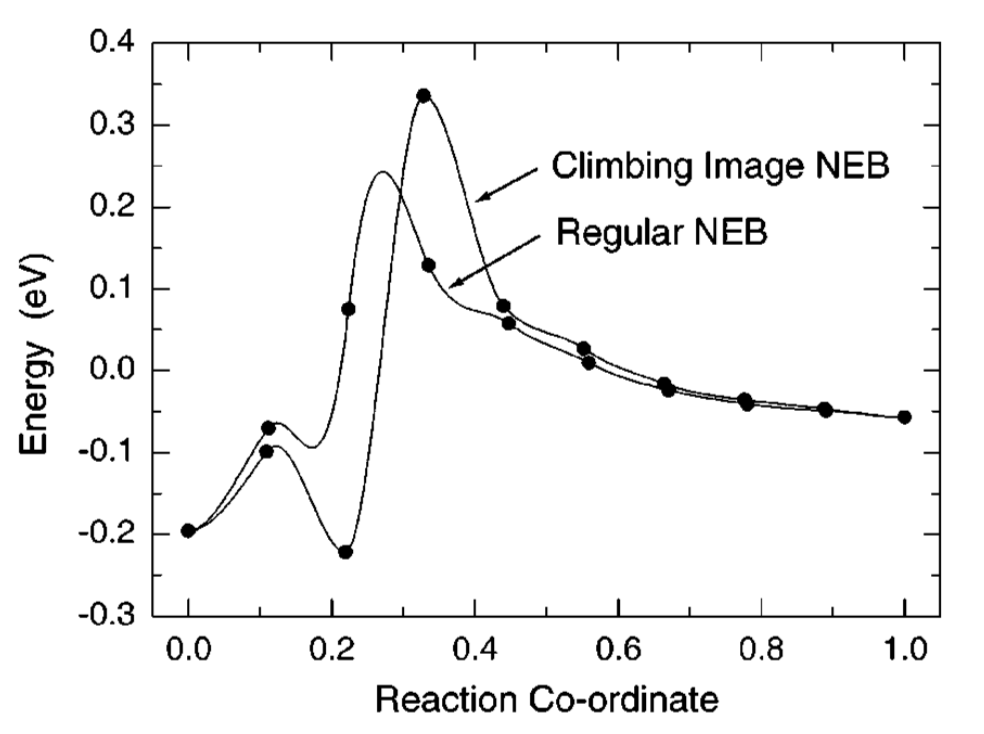
\includegraphics[width=0.5\textwidth]{./figures/DFT/ci-neb.png} 
\caption{\label{dft:fig-neb_climbing} \gls{NEB} calculation of the minimum energy path 
for \ce{CH4} dissociative adsorption on a Ir(111) surface, using both the 
regular \gls{NEB} algorithm as well as the climbing image 
modification.~\cite{Henkelman2000a}} 
\end{figure} 
 
\printbibliography 
\end{refsection} 
